%%%%%%%%%%%%%%%%%%%%%%%%%%%%%%%%%%%%%%%%%%%%%%%%%%%%%%%%%%%%%%%%%%%%%%%%
% \documentclass[preprint,12pt]{elsarticle}
\documentclass[final,12pt]{elsarticle}
%% \documentclass[final,1p,times]{elsarticle}
%% \documentclass[final,1p,times,twocolumn]{elsarticle}
%% \documentclass[final,3p,times]{elsarticle}
%% \documentclass[final,3p,times,twocolumn]{elsarticle}
%% \documentclass[final,5p,times]{elsarticle}
%% \documentclass[final,5p,times,twocolumn]{elsarticle}
%%%%%%%%%%%%%%%%%%%%%%%%%%%%%%%%%%%%%%%%%%%%%%%%%%%%%%%%%%%%%%%%%%%%%%%%
\usepackage{amsmath}
\usepackage{amssymb}
\usepackage{amsthm}
\usepackage{wasysym}

\usepackage{array}
\usepackage{booktabs}
\usepackage{caption}
\usepackage{subcaption}
\usepackage{tabularx}
\usepackage{tabularray}
\usepackage{multirow}

\usepackage{graphicx}
\usepackage{calc}

\usepackage{pdflscape}
\usepackage{lineno}
% \linenumbers

\usepackage[linesnumbered, ruled, vlined, noline]{algorithm2e}
%%%%%%%%%%%%%%%%%%%%%%%%%%%%%%%%%%%%%%%%%%%%%%%%%%%%%%%%%%%%%%%%%%%%%%%%
\journal{Knowledge-based Systems}
\begin{document}
\begin{frontmatter}

%% Title, authors and addresses
%% use the tnoteref command within \title for footnotes;
%% use the tnotetext command for theassociated footnote;
%% use the fnref command within \author or \affiliation for footnotes;
%% use the fntext command for theassociated footnote;
%% use the corref command within \author for corresponding author footnotes;
%% use the cortext command for theassociated footnote;
%% use the ead command for the email address,
%% and the form \ead[url] for the home page:
\title{DWISTGNN: Dynamic Spatio-Temporal Graph Neural Network 
with Wavelet Interaction for Multivariate Time Series Forecasting}
\author[NUE]{Zhang Fengchen\corref{cor}}
\cortext[cor]{Corresponding author}
\ead{21101002@nue.edu.cn}
\author[THU]{Sun Fuchun}
\author[NUE]{Lyu Xiao}
\author[NUE]{Zhang Xian}
\author[NUE]{Sun Lidong}

\affiliation[NUE]{
  organization={College of Electronic Engineering}, 
  addressline ={Naval University of Engineering}, 
  city        ={Wuhan}, 
  postcode    ={430030}, 
  state       ={Hubei}, 
  country     ={China}}
\affiliation[THU]{
  organization={Department of Computer Science and Technology}, 
  addressline ={Tsinghua University}, 
  city        ={Haidian}, 
  postcode    ={100084}, 
  state       ={Beijing}, 
  country     ={China}}
%%%%%%%%%%%%%%%%%%%%%%%%%%%%%%%%%%%%%%%%%%%%%%%%%%%%%%%%%%%%%%%%%%%%%%%%
%% Abstract
\begin{abstract}  % 
Multivariate Time Series (MTS) forecasting 
acts a vital role in numerous real-life scenarios.  % MTS
The emerging Spatio-Temporal Graph Neural Networks (STGNNs) 
have achieved brilliant progress by simultaneously 
modeling inter spatial relations between variates as a graph structure 
and capturing intra temporal patterns of series.  % STGNNs
However, the evolving spatial relations 
and the non-stationary temporal patterns 
pose challenges to accurate forecasting of MTS.  % challenges
To tackle these issues, we introduce a model named 
Dynamic Spatio-Temporal Graph Neural Network with Wavelet Interaction (DWISTGNN).  % DWISTGNN
The Dynamic Graph Construction (DGC) module establishes the evolving graph structure 
by integrating learnable embeddings and dynamic node features.  % DGC
The Data Transform (DT) module 
first converts the input representation 
from time domain into frequency domain 
by utilizing Discrete Wavelet Transform (DWT) 
and then encodes the data with time position embeddings.  % DT
The Frequency Interaction (FI) module facilitates deep interaction 
between different decomposed components 
to extract hidden spatio-temporal features.  % FI
Abundant experiments are performed on eight benchmark datasets 
and significant performance reveals the effectiveness of the proposed model.
Relevant codes and data are accessible at https://github.com/fczhang0606.  % experiments
\end{abstract}
%%%%%%%%%%%%%%%%%%%%%%%%%%%%%%%%%%%%%%%%%%%%%%%%%%%%%%%%%%%%%%%%%%%%%%%%
%% Keywords
\begin{keyword}  % 
MTS forecasting 
\sep dynamic graph construction 
\sep discrete wavelet transform 
\sep frequency interaction
\end{keyword}
%%%%%%%%%%%%%%%%%%%%%%%%%%%%%%%%%%%%%%%%%%%%%%%%%%%%%%%%%%%%%%%%%%%%%%%%
\end{frontmatter}
%%%%%%%%%%%%%%%%%%%%%%%%%%%%%%%%%%%%%%%%%%%%%%%%%%%%%%%%%%%%%%%%%%%%%%%%
%%%%%%%%%%%%%%%%%%%%%%%%%%%%%%%%%%%%%%%%%%%%%%%%%%%%%%%%%%%%%%%%%%%%%%%%
%% main text
%%%%%%%%%%%%%%%%%%%%%%%%%%%%%%%% 1-Introduction %%%%%%%%%%%%%%%%%%%%%%%%%%%%%%%%
\section{Introduction}
\label{sec-1}


% 1.1: MTS + MTSF
MTS refers to the structured data 
recorded during a period of time across multiple variates.  % MTS
As shown in \textbf{Fig.1}, 
when observed along the time axis, each variate's value 
changes according to certain temporal patterns.
When observed along the spatial axis, 
these variates often exhibit spatial correlations at each timestamp.  % spatial and temporal dependencies
MTS forecasting is a field 
that studies how to model spatio-temporal relations 
and predict the consequent sequence of the given time series.  % MTSF
Benefiting from the widely used low-cost sensors, 
MTS forecasting has found numerous applications in 
weather observation \cite{wang2024deepwind}\cite{xu2024dgformer}\cite{yang2024long}, 
energy prediction \cite{shen2024energy}\cite{zhuang2023multi}\cite{xing2023stcgcn}, 
traffic monitoring \cite{kong2023dynamic}\cite{li2024st}\cite{kong2024spatio} and so on.  % fields
\begin{figure}[h]  % [htbp]

  \centering

  \begin{minipage}{0.95\textwidth}
    \includegraphics[width=0.95\textwidth]{figs/fig_2.png}
  \end{minipage}%

  \caption{Spatial and Temporal Dependencies of MTS}

\end{figure}


% 1.2: historical review
Attempting to explore the intricate spatio-temporal relations, 
MTS forecasting methods have undergone several development periods.  % methods
Statistical methods 
\cite{box1976analysis}\cite{drucker1996support}\cite{zivot2006vector}\cite{chen2007narx}\cite{frigola2015bayesian} 
were first employed for the solution, 
but they fail to handle nonlinear patterns and unstable data in practice.  % statistical methods
Machine learning methods 
\cite{breiman2001random}\cite{regression1992introduction}\cite{zhang2003time} 
were then developed to model more complex relations, 
but they require a great deal of manual feature engineerings.  % machine learning rely heavily on
Recently, deep learning methods with all kinds of neural network variants 
have been widely utilized 
to capture high-dimensional non-linear dependencies.  % deep learning
Recurrent Neural Networks (RNNs) \cite{graves2012long}\cite{cho2014learning} 
employ an inner hidden state variable to store historical information, 
combing the outer current input to describe temporal patterns.  % RNNs
Convolutional Neural Networks (CNNs) \cite{lecun2002gradient} 
design a set of learnable kernels to pool multi-scale spatial features.  % CNNs
By the integration of RNNs and CNNs \cite{lai2018modeling}\cite{shih2019temporal}, 
MTS forecasting can be addressed 
through simultaneously capturing temporal patterns and spatial relations.  % RNNs+CNNs
However, CNNs are constrained to process regular grid structures 
which limits the model to solve more irregular and realistic problems.  % CNNs' limitation

The emerging Graph Neural Networks (GNNs) 
\cite{bruna2013spectral}\cite{defferrard2016convolutional}\cite{kipf2016semi} 
model the spatial relations of variates as a graph structure instead of grids, 
extending the data domain from Euclidean space to non-Euclidean space.  % GNNs
Taking the generated graph and MTS data as inputs, 
STGNNs \cite{jin2023spatio}\cite{corradini2024systematic} 
combine temporal unit (like RNNs) and spatial unit GNNs 
to predict the consequent sequence of the given time series, 
achieving outstanding performance for MTS forecasting.  % STGNNs


% 1.3.1: STGNNs-graph construction
From the viewpoint of graph construction, 
existing STGNNs can be classified into 
predefined-graph methods, adaptive-graph methods and dynamic-graph methods.  % 3
Predefined-graph methods \cite{li2017diffusion} assume that 
the graph structure is constant and can be constructed in advance by prior knowledge.
But generally there is a gap between prior knowledge and realistic spatial relations 
and these spatial relations are usually changing over time.  % predefined graph
Adaptive-graph methods \cite{wu2019graph}\cite{wu2020connecting}\cite{ta2022adaptive} 
utilize the learnable embeddings 
to infer the optimized graph structure within each training iteration, 
aiming to reduce this gap.
However, the adaptive graph structure is still considered static.  % adaptive graph
Dynamic-graph methods 
\cite{guo2021learning}\cite{lan2022dstagnn}\cite{ye2022learning}\cite{xia2025prost} 
can learn the evolving graph structure at every timestamp 
by introducing the time-varying input nodes' features.
But the constructed graphs across different timestamps 
can easily fall into unsmoothness 
due to discontinuous changes from nodes' features.  % dynamic graph

% 1.3.2: STGNNs-decomposition
From the viewpoint of series decomposition, 
STGNNs can be divided into odd-even decomposition methods, 
trend-seasonal decomposition methods and frequency decomposition methods.  % 3
Odd-even decomposition methods \cite{liu2022scinet} separate the original time series 
into two subseries based on their indices, 
both of which share common temporal patterns.  % odd-even
Trend-seasonal decomposition methods 
\cite{wu2021autoformer}\cite{wang2024timemixer}\cite{luo2024lsttn}\cite{seo2025st} 
disentangle the series 
into a trend- and a seasonal-component, 
respectively describing long- and short-term patterns.  % trend-seasonal
% shortcomings
Frequency decomposition methods 
\cite{cao2020spectral}\cite{zhou2022fedformer}\cite{yi2023frequency}\cite{xu2023fits}\cite{tian2025frera} 
decompose the time series 
into multiple frequency components, 
revealing distinct characteristics of different bands.
The usually adopted Fourier Transform (FT) 
is unsuitable for handling non-stationary data 
and can only provide global frequency information of the time series.  % frequency

% 1.3.3: STGNNs-interaction structure
From the viewpoint of model architecture, 
STGNNs can be grouped into 
coupled architecture methods and factorized architecture methods.  % 2
Coupled architecture methods \cite{li2017diffusion} 
embed the spatial modules into temporal modules 
to preserve the coupling relations.
But such a fusion mechanism lacks flexibility 
to capture complex spatio-temporal relations.  % coupled architecture
Factorized architecture methods \cite{zhao2019t}\cite{yu2017spatio} 
first separate spatial modules and temporal modules 
and then reorganize them in a serial or parallel manner.
The separated modules first extract spatial or temporal features independently 
and then deliver their outputs as inputs to the subsequent module.
Although factorized architecture is convenient to design, 
the interaction between the modules is insufficient.  % factorized architecture


% ideas
% Every node has its own temporal pattern of unique period and frequency 
% which is different from others'.
% That means, every node's value changes at a different rate in different phase 
% compared with other nodes.
% The whole time series' temporal pattern is a combined presentation 
% of all nodes' temporal patterns, 
% which is hard to describe with a simple mathematical function defined in global time domain 
% just like in traditional signal analysis field.


% 1.4: methods
To tackle the above issues, this work introduces a model named 
Dynamic Spatio-Temporal Graph Neural Network with Wavelet Interaction (DWISTGNN).  % DWISTGNN
The Dynamic Graph Construction (DGC) module 
learns the evolving graph structure at every timestamp 
by integrating the learnable embeddings 
to describe the initial specific graph structure and 
the dynamic node features 
to reflect the gradual changes of the graph evolution.  % DGC
The Data Transform (DT) module is introduced 
to first decompose the time series into multiple frequency components via DWT 
to reveal distinct characteristics of different bands 
and then encode the transformation results with time position embeddings.
The lower bands represent slower-varying smoothing trends, 
while the higher bands represent faster-varying drastic fluctuations.  % DT
The Frequency Interaction (FI) module is designed 
to promote the deep interaction between different frequency components.
Every component absorbs other component's information and 
all the processed components are then adaptively fused 
to acquire the representation for prediction.  % FI
% If there is N components, the FI module 
% will generate an interaction matrix $A_{mutal} \in R^{N \times N}$.
% The noise of the signal can be always filtered out during the high frequency processing part.


% 1.5: contributions
Main contributions of this work are: 
\begin{itemize}
\item
A model named Dynamic Spatio-Temporal Graph Neural Network 
with Wavelet Interaction (DWISTGNN) is introduced 
to address the graph learning problem, series analysis problem 
and spatio-temporal patterns extraction problem 
in multivariate time series forecasting field.  % model + problems + fields
\item
A joint framework is constructed 
consisting of Dynamic Graph Construction (DGC) module, 
Data Transform (DT) module and Frequency Interaction (FI) module 
to solve the aforementioned problems simultaneously 
and is trained in an end-to-end manner.  % architecture + module + end-to-end
\item
Abundant experiments are conducted on eight real-world datasets from various fields.
DWISTGNN achieves extraordinary performance, 
demonstrating the capability of the model.  % experiments + performance
\end{itemize}
%%%%%%%%%%%%%%%%%%%%%%%%%%%%%%%% 1-Introduction %%%%%%%%%%%%%%%%%%%%%%%%%%%%%%%%


%%%%%%%%%%%%%%%%%%%%%%%%%%%%%%%% 2-Related Work %%%%%%%%%%%%%%%%%%%%%%%%%%%%%%%%
\section{Related Work}
\label{sec-2}


\subsection{Multivariate Time Series Forecasting}
\label{subsec-2.1}


% 2.1.0: time series + forecasting
A time series defines a cluster of sampling points 
measured and indexed in sequential order, 
depicting the changing patterns of one or more variates.  % time series
A time series forecasting model 
aims to mine these underlying patterns from historical observations 
and analyze the future series.  % forecasting


% 2.1.1: statistical methods
Statistical methods are the earliest approaches for time series forecasting.  % statistical methods
Derived from autoregressive, moving average 
and their combination ARMA, 
autoregressive integrated moving average (ARIMA) \cite{box1976analysis} 
applied Box-Jenkins modeling methodology 
achieving a good performance for linear univariate time series.  % ARIMA
By treating the prediction as a classical regression task, 
support vector regression (SVR) \cite{drucker1996support} is also employed 
for univariate forecasting.  % SVR
As a generalization of AR-based methods, 
vector autoregression (VAR) \cite{zivot2006vector} was first applied 
for multivariate time series forecasting.  % VAR
The models mentioned above all assume that 
there are only linear relations among the time series, 
which becomes the major limitation of these models.  % linear assumption
More efforts are then shifted to the kernel methods \cite{chen2007narx} 
and Gaussian Processes (GP) \cite{frigola2015bayesian} to capture non-linearity.  % kernel + GP


% 2.1.2: ml + dl
Machine learning methods like 
Random Forest Regression (RFR) \cite{breiman2001random} 
and K-Nearest Neighbors (KNN) \cite{regression1992introduction}, 
were then developed to model more complex relations.  % machine learning
They are more effective than the traditional groups, 
while requiring much effort to design manual features.  % feature engineering
Based on the theory that any mathematical function can be approximated by neural networks, 
deep learning methods are powerful tools to explore the non-linear relations.  % deep learning
VARMLP \cite{zhang2003time} proposes a combined model 
integrating ARIMA and ANN 
to reduce the prediction error.  % VARMLP
RNNs like LSTM \cite{graves2012long} and GRU \cite{cho2014learning} 
are widely applied to model temporal patterns.  % RNNs
CNNs \cite{lecun2002gradient} 
are usually employed to extract the spatial dependencies.  % CNNs
LSTNet \cite{lai2018modeling} utilizes 1-D convolutional filters 
to uncover both variates' spatial relations and short-term temporal patterns 
and simultaneously employs RNN layers to model long-term temporal patterns.  % LSTNet
TPA-LSTM \cite{shih2019temporal} integrates LSTM 
with an attention mechanism 
to address long-range forecasting and 
identify the principal temporal patterns.  % TPA-LSTM
However, costly RNNs accumulate errors with every step due to iterative training 
and CNNs restrict the model to only process the regular grid structures, 
both of which constrain the development of the model.  % RNNs/CNNs' limitations


% 2.1.3: GNN + STGNN
A graph is a non-Euclidean data structure 
which is better suited for modeling irregular spatial relations in realistic scenarios.  % graph
GNNs \cite{bruna2013spectral}\cite{defferrard2016convolutional}\cite{kipf2016semi} 
are a cluster of models specifically operating on graph data.
Through an information exchanging process, 
nodes iteratively aggregate messages from their neighbors 
and update their own embeddings to incorporate both local and global information.  % GNNs
MTS forecasting can be formulated in a graph perspective naturally.
At every timestamp, variates are treated as nodes 
and hidden dependencies are established as edges.
As time goes by, both the values of the nodes and 
the strength of their connections change dynamically.  % MTS from graph perspective
STGNNs have been successfully employed for MTS forecasting in many fields 
\cite{jin2023spatio}\cite{corradini2024systematic}.  % STGNNs' review
However, significant challenges remain 
for better performance and broader applications.  % challenges


\subsection{Spatio-Temporal Graph Neural Networks}
\label{subsec-2.2}


% definition + characteristics + streams
STGNN is a specialized neural network architecture 
simultaneously performing 
graph convolution for capturing non-Euclidean spatial dependencies 
and temporal modeling for capturing dynamic evolution patterns 
to learn the node representations to accomplish downstream tasks.  % definition
The fundamental difference between STGNNs and traditional methods 
lies in the former's unified framework's ability 
to jointly extract spatio-temporal features, 
rather than analyzing spatial and temporal dependencies separately.  % characteristics
Looking back along the timeline, 
the evolution of STGNNs can be classified into three main streams.  % streams


% challenge-1: graph construction
According to the mined graph structure, 
STGNNs can be categorized into 
predefined-graph methods, adaptive-graph methods and dynamic-graph methods.  % 3
The predefined-graph methods build graph structures 
on the basis of prior knowledge like physical distance, node similarity and so on.  % predefined-graph
DCRNN \cite{li2017diffusion} extracts a directed weighted graph derived from the traffic network, 
describing asymmetric relations and connection strengths between nodes.  % DCRNN
The adaptive-graph methods still assume that the graph structure is static 
but acknowledge that prior knowledge can't fully represent the graph structure 
and try to bridge this gap in an adaptive manner.  % adaptive-graph
GWN \cite{wu2019graph} combines a predefined graph structure with an adaptive matrix 
which is generated by learnable embeddings to explore the unknown part of the structure.  % GWN
MTGNN \cite{wu2020connecting} further utilizes the learnable embeddings 
to represent the entire graph structure.  % MTGNN
At every timestamp, the better-learned graph matrix 
participates into the spatial relation extraction and 
the optimal graph structure can be obtained when the training ends.  % adaptive graph evolution
In realistic applications, the spatial relations between variates 
usually evolve over time, beyond static model's expressing ability.
To overcome this limitation, some dynamic-graph methods 
bring in time-varying nodes' features to generate the dynamic graph matrix.  % dynamic-graph
ASTGNN \cite{guo2021learning} developes a Dynamic Graph Convolution Net (DGCN) 
to measure relation strength adaptively.  % ASTGNN
DSTAGNN \cite{lan2022dstagnn} extracts the spatio-temporal aware distance (STAD) 
from historical data and 
uses the Wasserstein Distance to calculate the differences of probability distribution 
to construct the spatio-temporal aware graph.  % DSTAGNN
ESG \cite{ye2022learning} designs an Evolving Graph Structure Learner (EGL) 
that both considers the current dependency 
and the latest graph structure 
to recursively construct dynamic graph matrices.  % ESG


% challenge-2: series decomposition
According to the form of decomposed series, 
STGNNs can be categorized into 
odd-even decomposition methods, 
trend-seasonal decomposition methods and frequency decomposition methods.  % 3
SCINet \cite{liu2022scinet} implements a recursive architecture 
by decomposing the time series into odd- and even-subseries, 
introducing interactive learning to facilitate information exchange.  % SCINet
Autoformer \cite{wu2021autoformer} disentangles the series into a trend- and seasonal-component 
for capturing long- and short-term patterns respectively 
and incorporates an Auto-Correlation mechanism 
to discover dependencies by aggregating representations at subseries level.  % Autoformer
D2STGNN \cite{shao2022decoupled} proposes a Decoupled Spatio-Temporal Framework (DSTF) 
that decomposes traffic signals into diffusion and inherent components 
and employs an Estimation Gate to dynamically evaluate the ratio between them.  % D2STGNN
While the above methods handle time series forecasting in time domain, 
there are other works exploring solutions in frequency domain.  % time domain -- frequency domain
StemGNN \cite{cao2020spectral} 
first converts the series of each variate to spectral domain 
for orthogonality by leveraging a graph Fourier operation 
and then shifts the results to frequency domain.  % StemGNN
FEDFormer \cite{zhou2022fedformer} designs a Frequency Enhanced Block (FEB) 
to project the input series to frequency space 
and utilizes a Frequency Enhanced Attention (FEA) 
to transform the Q, K and V via Fourier Transform or Wavelet Transform 
to simulate a traditional attention process.  % FEDFormer
STWave \cite{fang2023spatio} disentangles the non-stationary time series 
into different frequency components using DWT 
and adopts a dual-channel encoder to process the components separately.  % STWave


% challenge-3: model architecture
According to the model architecture, 
STGNNs can be categorized into 
coupled architecture methods and factorized architecture methods.  % 2
In coupled architecture methods, 
spatial modules are usually integrated into temporal modules.  % coupled architecture
DCRNN \cite{li2017diffusion} 
embeds a graph diffusion convolution operator 
into GRU instead of standard multiplications 
to couple spatial-temporal relations.  % DCRNN
In factorized architecture methods, 
spatial and temporal modules are treated as separate blocks 
that exchange features with each other in a serial or parallel way.  % factorized architecture
T-GCN \cite{zhao2019t} adopts a serial manner by employing GRUs for temporal modeling.
The interfaces of each GRU include 
both the output from previous GRU 
and the output from a spatial GCN layer, 
forming a recursive and sequential structure.  % serial T-GCN
STGCN \cite{yu2017spatio} takes a parallel way to capture temporal patterns 
using 1-D causal convolution.
Within a single step, the convolution operation can be implemented 
simultaneously at every timestamp position 
by considering both previous and current timestamp states.  % parallel STGCN
To address shallow interaction limitation in factorized architecture methods, 
STIDGCN \cite{liu2024spatial} introduces a binary tree structure 
to perform hierarchical interactive learning between modules, 
enabling the identification of deeper spatio-temporal patterns.  % STIDGCN
%%%%%%%%%%%%%%%%%%%%%%%%%%%%%%%% 2-Related Work %%%%%%%%%%%%%%%%%%%%%%%%%%%%%%%%


%%%%%%%%%%%%%%%%%%%%%%%%%%%%%%%% 3-Preliminary %%%%%%%%%%%%%%%%%%%%%%%%%%%%%%%%
\section{Preliminary}
\label{sec-3}


Key background knowledge is provided to facilitate comprehension 
and \textbf{Table 1} lists the notations employed.  % 


\subsection{Definition: Dynamic Graph}
\label{subsec-3.1}


A dynamic graph is formulated as $G(t) = (V(t), E(t), A(t))$ 
where $V(t)$ denotes the set of nodes (variates), 
$E(t)$ denotes the set of edges and $A(t)$ denotes the dynamic adjacency matrix 
which describes the instantaneous connections between nodes at timestamp $t$.  % G(t)

Assuming $V(t)$ is constant in this work, namely $V(t) = V \in R^{N}$.
$N$ denotes the fixed number of nodes.  % V(t)
% formulation env
In contrast, the set of edges $E(t)$ always changes, 
resulting in a dynamic graph represented as $A(t) \in R^{N \times N}$.  % E(t) + A(t)


\subsection{Problem formulation}
\label{subsec-3.2}


MTS can be denoted as 
a sequence of $T$ timestamps of observations across multiple variates 
$X = \{ X_1, X_2, ... , X_T \} \in R^{D \times N \times T}$.
$X_t \in R^{D \times N}$ is the value matrix at timestamp $t$ 
of all $N$ variates with $D$ feature dimension.
For a certain task, $N$ and $D$ are fixed and $t \in T$.  % MTS: X

We set an observation window $W$ for historical time series 
and a forecasting horizon $H$ for prediction.  % W + H
The historical series is $W_{t} = \{ X_{t-W+1:t} \}$  % series - series
and the forecasting series is $H_{t} = \{ \widehat{X}_{t+1:t+H} \}$.  % W(t) + H(t)

Given the actual values $Y = \{ X_{T+1:T+H} \}$, 
the forecasting task falls into two categories.  % 2 types
Single-step task 
targets to forecast $\widehat{Y}_{s} = \{ \widehat{X}_{T+H} \}$ 
at specific timestamp $T+H$ 
and multi-step task 
targets to forecast $\widehat{Y}_{m} = \{ \widehat{X}_{T+1:T+H} \}$ 
within a range $H$ of timestamps.

The proposed model equals building an approximation 
$\widehat{Y} = model(X, \Theta)$.
$\Theta$ is the trainable parameter set.
\begin{equation}
  \begin{aligned}
    \Theta^{\star} = \underset{\Theta}{\arg\min} LOSS(Y, model(X, \Theta))
  \end{aligned}
\end{equation}


\subsection{Wavelet Transform}
\label{subsec-3.3}


Wavelet Transform (WT) \cite{daubechies1992ten} was proposed 
as a mathematical tool for signal analysis 
by computing the similarity between the signals and a set of math functions 
which are modified through scaling and translation based on the wavelet basis.  % WT
WT surpasses the widely adopted Fourier Transform (FT) 
as it supplies unified information in both time and frequency dimension, 
while FT can only offer a global frequency distribution 
without any time localization.  % information: time + frequency

WT of a signal $\textbf{x}$ is expressed as: 
$$WT(x, s, \delta) = <x, \phi_{s, \delta}> = 
\frac{1}{\sqrt{s}} \int x(t) \phi^{\ast} (\frac{t-\delta}{s}) dt$$ 
where $s>0$ is the scale parameter, $\delta$ is the translation parameter 
and $\phi^{\ast}$ is the wavelet basis.  % WT

Continuous Wavelet Transform (CWT) analyzes signals 
across all possible scales and translations, 
ideal for detailed continuous time-frequency studies.  % CWT
Discrete Wavelet Transform (DWT) adopts discrete scales and translations as parameters, 
having an advantage of computational efficiency in realistic applications.  % DWT
The common used wavelet basis functions 
include Haar, Daubechies, Coiflet, Symlet and Meyer.  % wavelet basis


\begin{table}[h]  % [htbp]
\label{tab-1}

  \caption{\textbf{Notations}}
  \small
  \centering

  \begin{tabular}{|l|l|}
    \hline  \multicolumn{1}{|c|}{Notation}  & \multicolumn{1}{c|}{Definition}             \\
    \hline  $X$                             & the input multivariate time series          \\
    \hline  $X_{t}$                         & the input tensor extracted from X at timestamp $t$    \\
    \hline  $Y, \widehat{Y}$                & the ground truth and the predicted series   \\
    \hline  $\textbf{g}, \textbf{h}$        & low- and high-pass filters in DWT           \\
    \hline  $X_{0, l}, X_{0, h}$            & reconstructed components after DWT and IDWT \\
    \hline  $I_{day}, I_{week}$             & the day and week time indexing vectors      \\
    \hline  $W_{day}, W_{week}$             & the day and week learnable projectors       \\
    \hline  $E_{day}, E_{week}$             & the day and week embedding tensors          \\
    \hline  $E_{time}$                      & the time embedding tensor                   \\
    \hline  $X_{l}, X_{h}$                  & frequency components encoded with time embeddings     \\
    \hline  $E_{s}$                         & the learnable embedding for specific graph construction  \\
    \hline  $A_{s}$                         & the specific graph                          \\
    \hline  $A_{d}$                         & the gradual changing graph                  \\
    \hline  $\Delta A$                      & the compensatory graph                      \\
    \hline  $A$                             & the entire dynamic graph                    \\
    \hline  $X_{l}^{(2)}, X_{h}^{(2)}$      & frequency components after two rounds of interaction  \\
    \hline
  \end{tabular}

\end{table}
%%%%%%%%%%%%%%%%%%%%%%%%%%%%%%%% 3-Preliminary %%%%%%%%%%%%%%%%%%%%%%%%%%%%%%%%


%%%%%%%%%%%%%%%%%%%%%%%%%%%%%%%% 4-Methodology %%%%%%%%%%%%%%%%%%%%%%%%%%%%%%%%
\section{Methodology}
\label{sec-4}


\subsection{Architecture}
\label{subsec-4.1}


DWISTGNN adopts an encoder-decoder design, 
as displayed in \textbf{Fig.2}.  % architecture
The encoder comprises most of the proposed modules 
to refine the input into deeper semantic representations.  % encoder
The decoder then accepts these intermediate representations as input 
to generate the final predictions.  % decoder

In the first stage, the raw input series 
is decomposed into two frequency components by applying DWT twice and IDWT.
Each component then undergoes a position embedding process 
to incorporate temporal knowledge for enhancing periodicity.  % PT
Simultaneously, the raw input series is also lead to 
the DGC module 
to build the dynamic graph structure.  % DGC
In the second stage, 
the time-embedded frequency components 
and the generated dynamic graph adjacency matrix 
are both utilized by the FI module 
to carry out a two-round interactive learning process.  % FI
Subsequently, the components that have fully exchanged features with each other 
are adaptively fused to obtain the integrated representation.  % adaptive fusion
Finally, the decoder employs a GLU unit 
to selectively filter information from the integrated representation.  % GLU
The predicted output is obtained after a regression layer 
to align with the horizon.  % Regression
\begin{figure}[h]  % [htbp]

  \centering

  %\begin{minipage}{0.95\textwidth}
    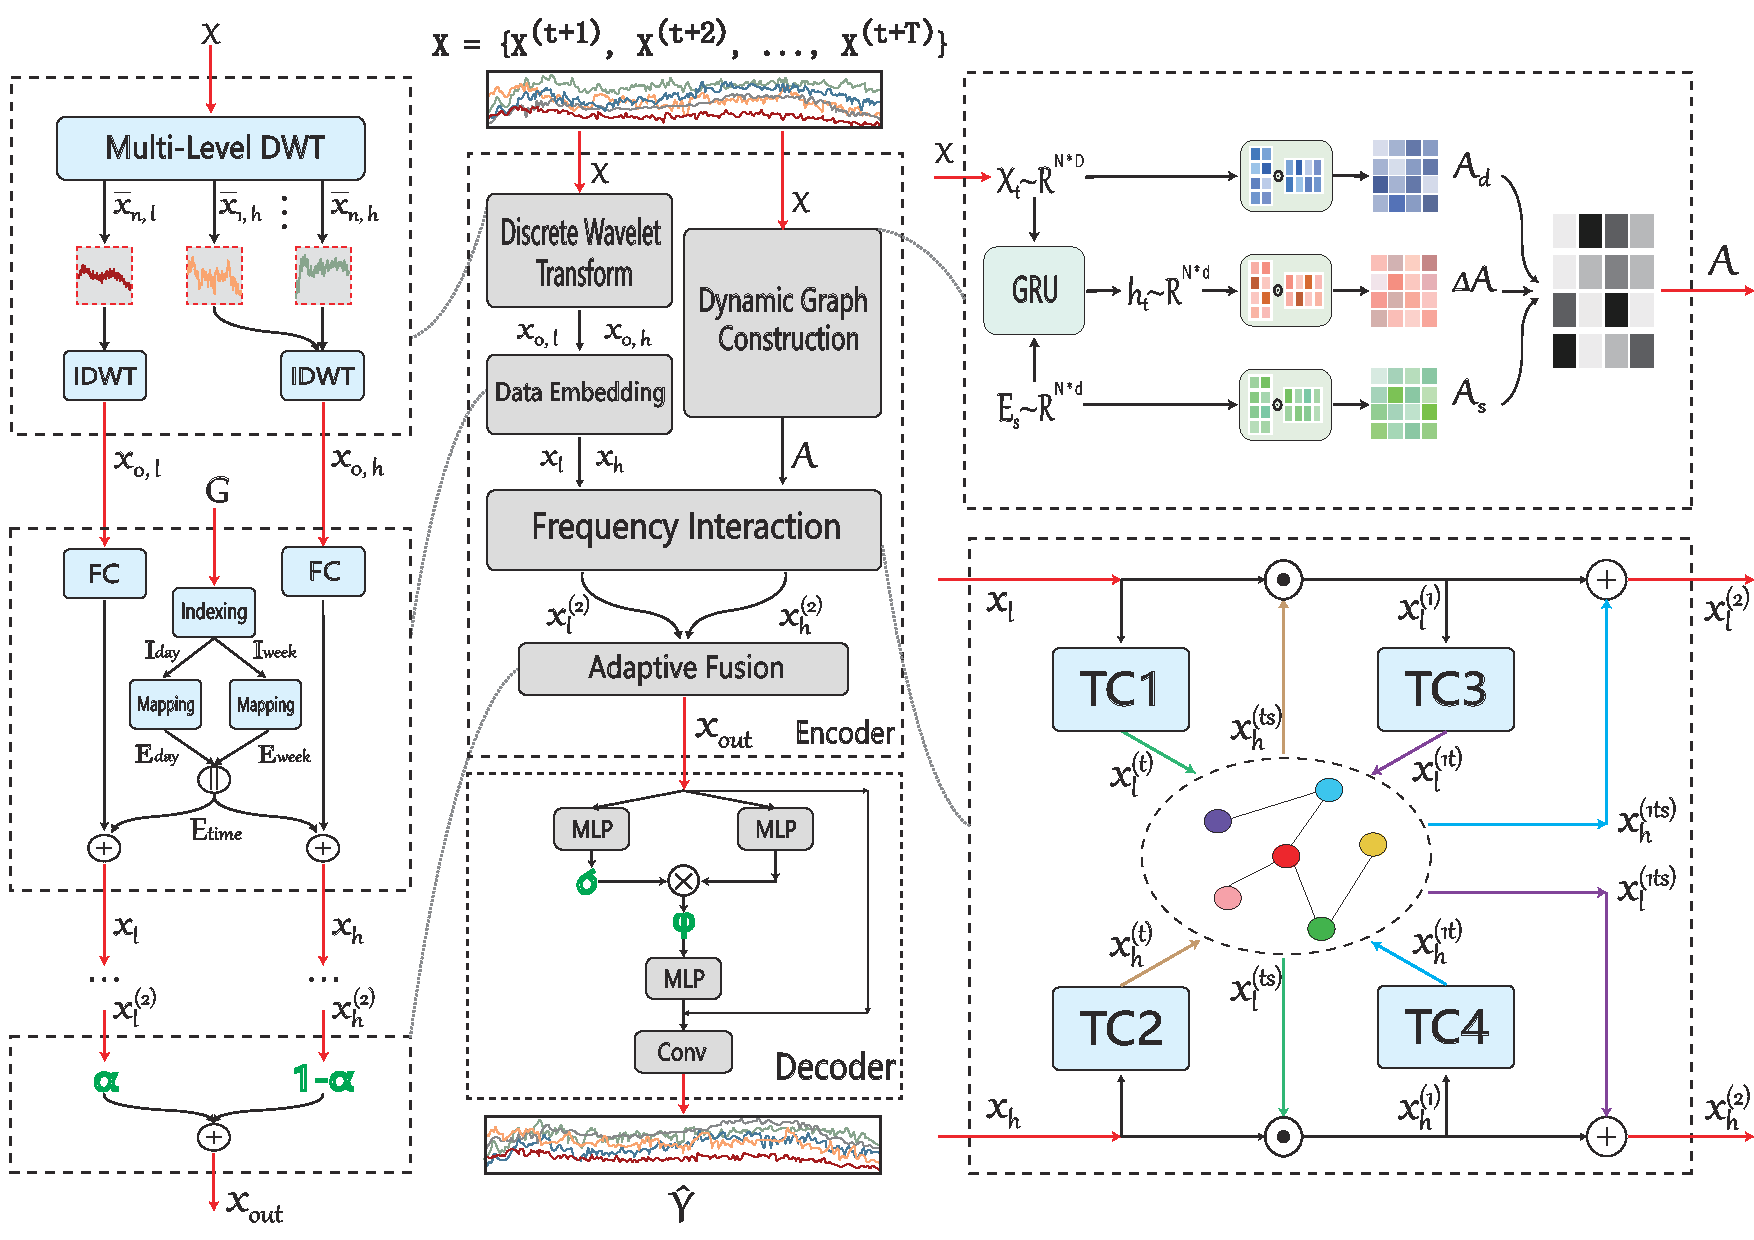
\includegraphics[width=0.98\textwidth]{figs/fig_1.png}
  %\end{minipage}%

  \caption{Overview Framework of DWISTGNN}

\end{figure}


\subsection{Data Transform}
\label{subsec-4.2}


\subsubsection{DWT and Inverse DWT}
\label{subsubsec-4.2.1}


DWT can be performed multiple times recursively.
With each iteration, 
the low- and high-pass decomposition filters $\textbf{g}$ and $\textbf{h}$ 
are used to decompose the input  
into components of distinct resolutions.  % DWT iteration
The results filtered by two filters are respectively denoted as 
$cA$ (Approximation Coefficients) and 
$cD$ (Detail Coefficients).  % Approximation + Details
The approximation coefficients $cA$ 
represent the coarse-grained patterns revealing the overall trend, 
while the detail coefficients $cD$ 
depict the fine-grained details of the signal.  % characteristics of cA and cD

DWT can be formulated as $cD_{l}$, $cA_{l}$ = DWT($cA_{l-1}$).
\begin{equation}
  \begin{aligned}
    cD_{l} &= \textbf{h} \star cA_{l-1}
            = \sum_{\lambda=1}^{\Lambda} h[2s-\lambda] cA_{l-1}[\lambda] 
              \quad s = 1, 2, ..., \frac{\Lambda}{2}  \\
    cA_{l} &= \textbf{g} \star cA_{l-1}
            = \sum_{\lambda=1}^{\Lambda} g[2s-\lambda] cA_{l-1}[\lambda] 
              \quad s = 1, 2, ..., \frac{\Lambda}{2}  \\
  \end{aligned}
\end{equation}
where $l$ indicates the $l$-th decomposition, 
$\Lambda$ represents the length of $cA_{l-1}$, 
$s$ represents the scale and $cA_{0} = \textbf{x}$.  % DWT

Given the raw input data $X \in R^{D \times N \times T}$, 
DWISTGNN conducts DWT twice 
to derive the approximation coefficient and multiple detail coefficients, 
listed as $\{X_{2, l}, X_{2, h}, X_{1, h}\}$: 
\begin{equation}
  \begin{aligned}
    X_{1, l} &= \textbf{g} \star X  \\
    X_{1, h} &= \textbf{h} \star X  \\
    X_{2, l} &= \textbf{g} \star X_{1, l}  \\
    X_{2, h} &= \textbf{h} \star X_{1, l}  \\
  \end{aligned}
\end{equation}  % X -> X1l/X1h -> X2l/X2h


The standard Inverse DWT (IDWT) is used 
to recover the approximation coefficients 
of the higher-level signal from its decomposed components 
and can be defined as 
\begin{equation}
  \begin{aligned}
    \widehat{cA_{l-1}} &= IDWT( \widehat{cD_{l}}, \widehat{cA_{l}} )  \\
                       &= \tilde{\textbf{h}} \star \widehat{cD_{l}} 
                        + \tilde{\textbf{g}} \star \widehat{cA_{l}}  \\
  \end{aligned}
\end{equation}  % IDWT
where $\tilde{\textbf{g}}$ and $\tilde{\textbf{h}}$ are reconstruction filters.
The original $\tilde{\textbf{x}}$ is recovered 
by applying IDWT recursively on all decomposed components.  % IDWT

DWISTGNN divides the decomposed coefficients into two parts 
to apply IDWT separately.  % IDWT parts
One part recorded as $\{ X_{2, l}, 0, 0 \}$ 
includes the approximation coefficient only 
and is padded with zeros to align with the original list's length 
to reconstruct $X_{0, l}$.  % cA only
The other part recorded as $\{ 0, X_{2, h}, X_{1, h} \}$ 
contains all detail coefficients 
and is also padded with zeros accordingly 
to reconstruct $X_{0, h}$.  % cD only
Theoretically, the original signal $\textbf{x}=X_{0, l}+X_{0, h}$, 
in which $X_{0, l}$ and $X_{0, h}$ respectively 
convey the low- and high-resolution information.  % 
\begin{equation}
  \begin{aligned}
    X_{0, l} &= W^{\tilde{\textbf{g}}} 
                ( \tilde{\textbf{g}} \star 
                ( \tilde{\textbf{g}} \star X_{2, l} )) 
                + b^{\tilde{\textbf{g}}}  \\
    X_{0, h} &= W^{\tilde{\textbf{h}}} 
                ( \tilde{\textbf{g}} \star (\tilde{\textbf{h}} \star X_{2, h}) + 
                  \tilde{\textbf{h}} \star X_{1, h}) 
                + b^{\tilde{\textbf{h}}}  \\
  \end{aligned}
\end{equation}  % X0l + X0h


\subsubsection{Position Embedding}
\label{subsubsec-4.2.2}


Position embedding integrates temporal location information into raw data 
to uncover the position relations of the time series.  % embedding of the time knowledge


First, we assign indexes of ``day'' and ``week'' 
to every timestamp position in the series, 
resulting in 
$I_{day}  \in R^{N \times T}$ and 
$I_{week} \in R^{N \times T}$.  % indexing vectors of day and week
\begin{equation}
  \begin{aligned}
    I_{day}  &= Duplicate(\{i \% G / G  \}_{i \in T})^{N} 
             &\quad \quad \in R^{N \times T}  \\
    I_{week} &= Duplicate(\{i // G \% 7 \}_{i \in T})^{N} 
             &\quad \quad \in R^{N \times T}  \\
  \end{aligned}
\end{equation}
$i$ denotes the index of timestamp.
$G$ denotes the granularity, namely the totality of timestamps in a day.
$I_{day}$ and $I_{week}$ denote 
which hour and day that every timestamp belongs to.  % indexing vectors


Then we define two learnable temporal projectors, i.e., 
$W_{day}  \in R^{C \times G}$ and 
$W_{week} \in R^{C \times 7}$ 
to learn the periodicities adaptively.  % adaptive projectors of day and week, W
$E_{day}  \in R^{C \times N \times T}$ and 
$E_{week} \in R^{C \times N \times T}$ 
are generated by indexing 
learnable embedding matrix $W_{day}$ and $W_{week}$ 
with every element of $I_{day}$ and $I_{week}$ respectively.  % E_day + E_week
% Using the element values of the index vector as indices, 
% retrieve the corresponding embedding vectors from the adaptive vector matrix to generate E.
$C$ represents the expanded dimension.
The combined temporal periodic embedding 
$E_{time} \in R^{C \times N \times T}$ is 
\begin{equation}
  \begin{aligned}
    E_{time} = (E_{day} + E_{week}) \quad \in R^{C \times N \times T}
  \end{aligned}
\end{equation}  % E(time)


Subsequently, the components 
$X_{0, l} \in R^{D \times N \times T}$, 
$X_{0, h} \in R^{D \times N \times T}$ ascend their dimension to 
$R^{C \times N \times T}$ 
to enrich semantic information 
through a fully connected layer respectively.  % D -- C
The final $X_{l}$ and $X_{h}$ are yielded 
by concatenating $E_{time}$ along the channel dimension 
to absorb the prior position information.  % X + E
\begin{equation}
  \begin{aligned}
    X_{l} &= (W_{l} X_{0, l}) || E_{time} 
          &\quad \in R^{2C \times N \times T}  \\
    X_{h} &= (W_{h} X_{0, h}) || E_{time} 
          &\quad \in R^{2C \times N \times T}  \\
  \end{aligned}
\end{equation}  % X = X + E(time)


\subsection{Dynamic Graph Construction}
\label{subsec-4.3}


Generally, the spatial relations between variates change over time, 
which start from an unknown specific graph structure 
and evolve to the present structure.  % dynamic graph = initial + changing
Assuming the change during this period is continuous, 
the current structure can be considered 
as a sum of three distinct structure components.  % 3
The initial specific graph structure component 
is optimized by the learnable embeddings.
The gradual changing graph component describing the evolution 
is captured by tracking the dynamic node-level inputs.  % initial + changing
A third compensatory component employs a GRU 
to integrate the two aforementioned components 
and applies a self-attention mechanism 
to ensure a smoother transition process.  % compensatory


To learn the initial specific graph, 
a trainable embeddings $E_{s} \in R^{d \times N}$ 
is employed to construct the structure adaptively.
The dimension $d$ is usually far less than $N$, 
helpful to reduce the computational cost.  % Es
The adjacency matrix of initial specific graph is inferred: 
\begin{equation}
  A_{s} = SoftMax(ReLU(E_{s} \cdot E_{s}^{'}))
\end{equation}
$E_{s}^{'}$ is the transpose of $E_{s}$.
ReLU blocks the weak connections 
and SoftMax normalizes the results.  % As


The gradual changes of the graph evolution 
can be associatied with the node-level inputs 
$X_{t} \in R^{D \times N}$. Similarly, 
\begin{equation}
  A_{d} = SoftMax(ReLU(X_{t} \cdot X_{t}^{'}))
\end{equation}  % Ad


By integrating the learnable embeddings dictionary $E_{s}$ 
and the dynamic node-level inputs $X_{t}$ 
with a gated mechanism, 
we can get a fused hidden representation 
$h_{t} \in R^{d \times N}$.  % ht
\begin{equation}
  \begin{aligned}
    r_{t}           &= \sigma(W_{r} \cdot E_{s} + U_{r} \cdot X_{t})  \\
    z_{t}           &= \sigma(W_{z} \cdot E_{s} + U_{z} \cdot X_{t})  \\
    \widehat{h_{t}} &= tanh(W_{h}   \cdot X_{t} + r_{t} (U_{h} \cdot E_{s}))  \\
    h_{t}           &= (1 - z_{t})  \cdot E_{s} + z_{t} \cdot \widehat{h_{t}}  \\
  \end{aligned}
\end{equation}

The hidden intermediate representation $h_{t}$ 
undergoes a self-attention 
to produce a dynamic compensatory matrix $\Delta A$.  % ht -> detA
\begin{equation}
  \begin{aligned}
    Q &= W_{q} \cdot h_{t}  \\
    K &= W_{k} \cdot h_{t}  \\
    V &= W_{v} \cdot h_{t}  \\
    \Delta A &= Dropout(\frac{Q \cdot K^{'}}{\sqrt{d}})  \\
  \end{aligned}
\end{equation}
where $K^{'}$ is the transpose of $K$ and 
$W_{q}$, $W_{k}$ and $W_{v}$ 
are linear projectors.  % self-attention


Finally, the dynamic adjacency matrix is generated 
by integrating the above three matrices.
\begin{equation}
  A = SoftMax(A_{s} + A_{d} + \Delta A)  \\
\end{equation}  % A


\subsection{Frequency Interaction}
\label{subsec-4.4}


\subsubsection{Frequency Temporal Convolution}
\label{subsubsec-4.4.1}


% The temporal convolution module applies 
% a set of standard dilated 1D convolution filters 
% to extract high-level temporal features.
% \begin{equation}
%   \begin{aligned}
    % z \star f_{1 \times k}(t) = \sum_{i=0}^{k-1} f_{1 \times k}(i) z(t - d \times i)  \\
    % z = concat(z \star f_{1 \times 2}, z \star f_{1 \times 3}, 
    %            z \star f_{1 \times 6}, z \star f_{1 \times 7})
%   \end{aligned}
% \end{equation}
% $ z \in R^{T} $ is the 1D sequence input.
% $ f_{1 \times k} \in R^{k} $ is the 1D convolution filter with kernel size k.
% d is the dilation factor.


Temporal Convolution (TC) aims to 
extract intra temporal patterns.  % TC
As shown in \textbf{Fig.2},  % 
four TC modules labeled as TC1, TC2, TC3 and TC4 are embedded into the FI module 
to jointly capture the global representation.  % 4*TC -- FI
Different labeled TC modules have different inputs and outputs, 
while all of them share the same structure.
TC is composed of two convolutional layers with different kernels: 
\begin{equation}
  \begin{aligned}
    H_{out} = \sigma(Conv_{2}(\sigma(Conv_{1}(H_{in}))))  \\
  \end{aligned}
\end{equation}
$H_{in}$ and $H_{out}$ represents the interfaces of TC 
and $\sigma$ is the activation function.  % TC = two layers of CNN


\subsubsection{Frequency Spatial Convolution}
\label{subsubsec-4.4.2}


Spatial Convolution (SC) adopts a hix-hop graph convolution 
aiming to incorporate a variate's feature with its neighbors' 
to extract the spatial relations.  % SC
\begin{equation}
  \begin{aligned}
    H^{(k)} &= (1 - \beta) A H^{(k-1)} + \beta H_{in}  \\
    H_{out} &= \sum_{k=0}^{K} W^{(k)} H^{(k)}  \\
  \end{aligned}
\end{equation}  % hix-hop
$H_{in} = H^{(0)}$ denotes the input of SC, 
usually fed directly by the previous TC.
$\beta$ is the controlled ratio 
to retain a portion of raw information.
$A$ is the dynamic adjacency matrix generated by the DGC module.
$K$ is the depth of propagation.


\subsubsection{Frequency Interaction and Fusion}
\label{subsubsec-4.4.3}


Frequency Interaction completes an exchange of spatio-temporal features 
between different frequency components.  % FI
The components obtained by data transform can be denoted as 
$X_{l} \in R^{2C \times N \times T}$ and 
$X_{h} \in R^{2C \times N \times T}$, 
which are inputs of the FI module.  % input: Xl + Xh
In the first round of interaction, 
each component absorbs the processed information 
from other components' spatio-temporal extraction $X_{*}^{(ts)}$.  % first round
Similarly in the second round of interaction, 
components obtained by the first round $X_{*}^{(1)}$ 
continuously incorporate information 
from other components' another extraction.  % second round
This two-round interaction promotes 
the deep multi-resolution spatio-temporal exchange 
of different components and can be defined as follows: 
\begin{equation}
  \begin{aligned}
    & X_{l}^{(ts)}  = tanh(SC(TC1(X_{l})))  \\
    & X_{h}^{(ts)}  = tanh(SC(TC2(X_{h})))  \\
    & X_{l}^{(1)}   = X_{h}^{(ts)} \otimes X_{l}  \\
    & X_{h}^{(1)}   = X_{l}^{(ts)} \otimes X_{h}  \\
    & X_{l}^{(1ts)} = tanh(SC(TC3(X_{l}^{(1)})))  \\
    & X_{h}^{(1ts)} = tanh(SC(TC4(X_{h}^{(1)})))  \\
    & X_{l}^{(2)}   = X_{h}^{(1ts)} \otimes X_{l}^{(1)}  \\
    & X_{h}^{(2)}   = X_{l}^{(1ts)} \otimes X_{h}^{(1)}  \\
  \end{aligned}
\end{equation}  % 


Different frequency components represent 
distinct temporal patterns in different bands.  % patterns
The fusion of the components represents 
holistic characteristics of the series.  % fusion of patterns
Since the amplitudes of the components are varisized and unknown, 
we adopt an adaptive fusion mechanism 
to integrate the components to reconstruct the time series.  % adaptive fusion
\begin{equation}
  \begin{aligned}
    X_{out} = sigmoid(\mu) X_{l}^{(2)} + (1-sigmoid(\mu)) X_{h}^{(2)}  \\
  \end{aligned}
\end{equation}
where $\mu$ is a learnable parameter to control the fusion ratio.


\subsection{Decoder}
\label{subsec-4.5}


The $X_{out}$ generated by the encoder 
first passes through a GLU, which processes the representation into two branches.
One branch is activated by a sigmoid function to produce a gating signal, 
which then selectively modulates the other branch's representation 
to filter out irrelevant information.  % GLU
The output of this gating operation 
is then integrated with the original input 
to mitigate the gradient vanishing problem.  % residual layer
Finally, a regression layer utilizing a convolution unit 
reduces the channel dimension from $2C$ to $H$ 
to match the forecasting horizon, 
yielding the final predictions.  % regression layer
The decoder can be formulated as follows: 
\begin{equation}
  \begin{aligned}
    \widehat{Y} = Conv(MLP(ReLU(\sigma(MLP(X_{out})) \otimes MLP(X_{out}))) + X_{out})  \\
  \end{aligned}
\end{equation}
$\widehat{Y} \in R^{N \times H}$ 
denotes the predicted time series.  % decoder


We choose RRSE loss 
as training objective for single-step forecasting task 
and MAE loss 
for multi-step forecasting task: 
\begin{equation}
  \begin{aligned}
    & LOSS_{s}(Y, X, \Theta) = RRSE(Y, \widehat{Y}_{s})  \\
    & LOSS_{m}(Y, X, \Theta) = MAE (Y, \widehat{Y}_{m})  \\
  \end{aligned}
\end{equation}
The definition of RRSE and MAE can be found in Experiment section 
and the detailed learning process of DWISTGNN 
is shown in \textbf{Algorithm 1}.


% https://blog.csdn.net/qq_43486745/article/details/124344365
\begin{algorithm}[h]  % [htbp]
\label{alg-1}


  \LinesNotNumbered
  \SetAlgoLined
  \caption{DWISTGNN}


  \KwIn{Dataset D}
  \textbf{Parameters:} 
  $wavelet$, $epoch$, $iter$, $B$, $W$, $H$, $C$, $d$, $K$, $dropout$, $\alpha$, $\gamma$  \\
  \KwOut{The learned DWISTGNN model}
  Init $E_{time}$, $E_{s}$ and $\Theta$ \;

  \For{$i \leftarrow 1$ \KwTo $epoch$}{
    \For{$j \leftarrow 1$ \KwTo $iter$}{

      Sample $X \in R^{B \times D \times N \times W}$, \ 
      $Y \in R^{B \times N \times H}$ from $D$  \;

      $X_{0, l}, X_{0, h}$ 
      \gets \{$X$\} 
      \hfill $\triangleright$ Eq.~(3)(5): DWT and IDWT

      $X_{l}, X_{h}$ 
      \gets \{$X_{0, l}, X_{0, h}, E_{time}$\}  \\
      \hfill $\triangleright$ Eq.~(6)-(8): Position Embedding

      $A$ 
      \gets \{$X, E_{s}$\} 
      \hfill $\triangleright$ Eq.~(9)-(13): Dynamic Graph Construction

      $X_{l}^{(2)}, X_{h}^{(2)}$ 
      \gets \{$X_{l}, X_{h}, A$\}  \\
      \hfill $\triangleright$ Eq.~(14)-(16): Frequency Interaction

      $X_{out}$ 
      \gets \{$X_{l}^{(2)}, X_{h}^{(2)}$\} 
      \hfill $\triangleright$ Eq.~(17): Adaptive Fusion

      $\widehat{Y}$ 
      \gets \{$X_{out}$\} 
      \hfill $\triangleright$ Eq.~(18): Decoder

      $L$ 
      \gets \{$Y, \widehat{Y}$\} 
      \hfill $\triangleright$ Eq.~(19): Loss Function

      $\Theta$ 
      \gets \{$L, \alpha, \gamma$\} 
      \hfill $\triangleright$ Eq.~(1): Parameters Update

      $j \leftarrow j + 1$  \;
    }
    $i \leftarrow i + 1$  \;
  }

  \Return{$\Theta^{\star}$}  \;
\end{algorithm}
%%%%%%%%%%%%%%%%%%%%%%%%%%%%%%%% 4-Methodology %%%%%%%%%%%%%%%%%%%%%%%%%%%%%%%%


%%%%%%%%%%%%%%%%%%%%%%%%%%%%%%%% 5-Experiment %%%%%%%%%%%%%%%%%%%%%%%%%%%%%%%%
\section{Experiment}
\label{sec-5}


\subsection{General Settings}
\label{subsec-5.1}


\subsubsection{Dataset Statistics}
\label{subsubsec-5.1.1}


\textbf{Table 2} summarizes the corpus statistics 
for two benchmark dataset groups, 
i.e., single- and multi-step forecasting tasks.  % single + multi
Each dataset is chronologically split into 
training, validation, and test sets 
in a 6:2:2 ratio.  % partition
For single-step tasks, 
the look-back size is 168.
The prediction horizons in independent trained cases are set to 3/6/12/24 
and the prediction size is 1.  % W + H
For multi-step tasks, 
the look-back size is 12 
and the prediction series consists of 12 successive steps.  % W + H


% https://blog.csdn.net/everyxing1007/article/details/141892253
\begin{table}[h]  % [htbp]
\label{tab-2}

  \caption{\textbf{Dataset Statistics}}
  \tiny
  \centering
  \renewcommand{\arraystretch}{1.5}

  \begin{tabular}{|c|c|c|c|c|c|c|c|}
    \hline  Task Type & Dataset       & Partition       & Variates        & Timestamps 
                      & Granularity   & Input Size      & Predicted Size  \\
    \hline  \multirow{4}{*}{Single-step} 
                      & Electricity   & 0.6/0.2/0.2     & 321             & 26304 
                      & 1 h           & 168             & 3/6/12/24       \\
                      & Exchange-Rate & 0.6/0.2/0.2     & 8               & 7588 
                      & 1 day         & 168             & 3/6/12/24       \\
                      & Solar-Energy  & 0.6/0.2/0.2     & 137             & 52560 
                      & 10 mins       & 168             & 3/6/12/24       \\
                      & Traffic       & 0.6/0.2/0.2     & 862             & 17544 
                      & 1 h           & 168             & 3/6/12/24       \\
    \hline  \multirow{4}{*}{Multi-step} 
                      & PeMS03        & 0.6/0.2/0.2     & 358             & 26208 
                      & 5 mins        & 12              & 0-12            \\
                      & PeMS04        & 0.6/0.2/0.2     & 307             & 16992 
                      & 5 mins        & 12              & 0-12            \\
                      & PeMS07        & 0.6/0.2/0.2     & 883             & 28224 
                      & 5 mins        & 12              & 0-12            \\
                      & PeMS08        & 0.6/0.2/0.2     & 170             & 17856 
                      & 5 mins        & 12              & 0-12            \\
    \hline
  \end{tabular}

\end{table}


\begin{itemize}

\item \textbf{Electricity}:  % 
This dataset is a widely used benchmark particularly for energy consumption prediction.
The data recorded at 1-hour intervals from 321 clients 
spans from 2011 to 2014 and contains 26,304 timestamps.

\item \textbf{Exchange-Rate}:  % 
This dataset is a widely used benchmark particularly for financial data prediction.
The data recorded at 1-day intervals from 8 countries 
spans from 1990 to 2016 and contains 7,588 timestamps.

\item \textbf{Solar-Energy}:  % 
This dataset is a widely used benchmark particularly for renewable energy forecasting.
The data recorded at 10-minute intervals from 137 solar power facilities 
in Alabama in 2006 
contains 52,560 timestamps.

\item \textbf{Traffic}:  % 
This dataset is a widely used benchmark particularly for traffic flow forecasting.
The data recorded at 1-hour intervals from 862 detectors 
in San Francisco 
spans from 2015 to 2016 and contains 17,544 timestamps.


% https://nbsdc.cn/general/dataDetail?id=674b68dc195d2661e1ba4125&type=1
\item \textbf{PeMS03}:  % PeMS03
This dataset contains transportation data from Los Angeles.
The data collected at 5-minute intervals from 358 detectors 
spans from 2018.09.01 to 2018.11.30 
and includes 26,208 timestamps.

\item \textbf{PeMS04}:  % PeMS04
This dataset contains transportation data from San Francisco.
The data collected at 5-minute intervals from 307 detectors 
spans from 2018.01.01 to 2018.02.28 
and includes 16,992 timestamps.

\item \textbf{PeMS07}:  % PeMS07
This dataset contains transportation data from California District 7.
The data collected at 5-minute intervals from 883 detectors 
spans from 2017.05.01 to 2017.08.31 
and includes 28,224 timestamps.

\item \textbf{PeMS08}:  % PeMS08
This dataset contains transportation data from San Bernardino.
The data collected at 5-minute intervals from 170 detectors 
spans from 2016.07.01 to 2016.08.31 
and includes 17,856 timestamps.

\end{itemize}


\subsubsection{Hyperparameters and Metrics}
\label{subsubsec-5.1.2}


\textbf{Table 3} summarizes the hyperparameters used in DWISTGNN.  % Table 3
Epoch ($E$) limits the iterations to prevent overfitting.  % E
Wavelets including coif1, db1 and sym2 of distinct characteristics 
are used to implement DWT across different datasets.  % wavelet
The scale of Batch Size ($B$) affects the model's generalization.  % batch size
Window ($W$) refers to the length of the observed series.  % W
Horizon ($H$) indicates the steps ahead to be predicted.  % H
Channel ($C$) means the expanded dimensionality compared with the input.  % C
Dimension ($d$) corresponds to the dimensionality of the learnable graph embeddings.  % d
Diffusion Depth ($K$) determines the extent of neighborhood aggregation 
in diffusion convolution.  % K
Dropout rate is applied to mitigate overfitting.  % dropout
Learning Rate ($\alpha$) controls the step size during gradient descent.  % learning rate
Weight Decay ($\gamma$) serves as a regularization term 
that dynamically adjusts $\alpha$ 
to balance convergence speed and training stability.  % weight decay


The hardware environment of experiments 
consists of an Intel Core i9-13900KF CPU @ 3.0 GHz and 
an NVIDIA GeForce RTX 4090 GPU with 24 GB of memory.  % hardware environment
The software environment 
takes Python 3.8 and the PyTorch 1.12.1 framework.  % software environment


\begin{table}[h]  % [htbp]
\label{tab-3}

  \caption{\textbf{Hyperparameters}}
  \tiny
  \centering
  \renewcommand{\arraystretch}{1.5}

  \begin{tabular}{|c|c|c|c|c|c|c|c|c|}
    \hline  Hyperparameters   & Electricity & Exchange-Rate & Solar-Energy  & Traffic 
                              & PeMS03      & PeMS04        & PeMS07        & PeMS08  \\
    \hline  Wavelet           & db1         & db1           & sym2          & db1     
                              & db1         & db1           & coif1         & db1     \\
    \hline  $E$               & 1000        & 1000          & 1000          & 1000    
                              & 1000        & 1000          & 1000          & 1000    \\
    \hline  $B$               & 64          & 64            & 64            & 64      
                              & 96          & 96            & 96            & 96      \\
    \hline  $W$               & 168         & 168           & 168           & 168     
                              & 12          & 12            & 12            & 12      \\
    \hline  $H$               & 3/6/12/24   & 3/6/12/24     & 3/6/12/24     & 3/6/12/24 
                              & 0-12        & 0-12          & 0-12          & 0-12    \\
    \hline  $C$               & 64          & 32            & 64            & 128     
                              & 64          & 64            & 128           & 64      \\
    \hline  $d$               & 10          & 10            & 10            & 10      
                              & 10          & 10            & 10            & 10      \\
    \hline  $K$               & 2           & 1             & 2             & 2       
                              & 1           & 1             & 2             & 1       \\
    \hline  dropout           & 0.3         & 0.5           & 0.3           & 0.3     
                              & 0.5         & 0.5           & 0.5           & 0.5     \\
    \hline  $\alpha$          & 0.0001      & 0.0001        & 0.0001        & 0.0001  
                              & 0.0001      & 0.0001        & 0.0001        & 0.0001  \\
    \hline  $\gamma$          & 0.0005      & 0.0005        & 0.0005        & 0.0005  
                              & 0.0005      & 0.0005        & 0.0005        & 0.0005  \\
    \hline
  \end{tabular}

\end{table}


Supposing $\{ y = y_1, y_2, ..., y_n \}$ denotes the actual values, 
$\{ \widehat{y} = 
\widehat{y_1}, \widehat{y_2}, ..., \widehat{y_n} \}$ 
denotes the forecasted series 
and $\Psi$ denotes the sample set.

Mean Absolute Error (MAE)
$$ MAE(y, \widehat{y}) = 
\frac{1}{|\Psi|} 
\sum_{i \in \Psi} 
|y_i - \widehat{y_i}| $$

Mean Absolute Percentage Error (MAPE)
$$ MAPE(y, \widehat{y}) = 
\frac{1}{|\Psi|} 
\sum_{i \in \Psi} 
| \frac{y_i - \widehat{y_i}}{y_i} | $$

Root Mean Square Error (RMSE)
$$ RMSE(y, \widehat{y}) = 
\sqrt{ 
\frac{1}{|\Psi|} 
\sum_{i \in \Psi} 
(y_i - \widehat{y_i})^2 } $$

Root Relative Squared Error (RRSE)
$$ RRSE(y, \widehat{y}) = 
\sqrt{ 
\frac
{ \sum_{i \in \Psi} (y_i - \widehat{y_i})^2 }
{ \sum_{i \in \Psi} (y_i - \overline{\widehat{y}})^2 } } $$

Correlation Coefficient (CORR)
$$ CORR(y, \widehat{y}) = 
\frac
{ \sum_{i \in \Psi} 
(y_{i} - \overline{y}) 
(\widehat{y_{i}} - \overline{\widehat{y}}) }
{ \sqrt{ 
\sum_{i \in \Psi} 
(y_{i} - \overline{y})^2 
(\widehat{y_{i}} - \overline{\widehat{y}})^2 } } $$

Lower MAE, MAPE, RMSE and RRSE and 
higher CORR indicate better model performance.


\subsubsection{Baselines}
\label{subsubsec-5.1.3}


DWISTGNN is compared with the following baseline models.  \\


\noindent \textbf{Single-step Forecasting Model}
\begin{itemize}

\item AR \cite{box1976analysis}: 
A classical forecasting model 
that assumes the current value of a variate 
depends linearly on its own previous values 
plus a stochastic error term.

\item GP \cite{frigola2015bayesian}: 
It treats a time series as a sample from a Gaussian process 
and uses Bayes theorem 
to derive a posterior distribution for point forecasting.

\item VARMLP \cite{zhang2003time}: 
This hybrid time series forecasting model 
combines VAR and MLP, 
where the VAR component captures linear dependencies 
and the MLP component captures nonlinear dependencies.

\item RNN-GRU \cite{cho2014learning}: 
This network introduces gating mechanisms 
to address the constraints of traditional RNNs, 
like the vanishing gradient problem.

\item LSTNet \cite{lai2018modeling}: 
A method effectively analyzes both long- and short-term temporal dependencies 
by combining RNNs and CNNs.

\item TPA-LSTM \cite{shih2019temporal}: 
An advanced forecasting model 
that integrates LSTM with a Temporal Pattern Attention (TPA) mechanism, 
dynamically focusing on critical temporal patterns 
to enhance prediction accuracy.

\item MTGNN \cite{wu2020connecting}: 
A classical model equipped with a graph learning module 
that learns the relations between variates 
via a self-adaptive adjacency matrix.

\item Informer \cite{zhou2021informer}: 
A variant of Transformer 
to address high computational cost and memory usage 
by employing efficient attention mechanisms.

\item Autoformer \cite{wu2021autoformer}: 
By integrating decomposition and auto-correlation mechanisms, 
the model effectively captures complex temporal patterns.

\item GTS \cite{shang2021discrete}: 
GTS proposes a method 
for the joint learning 
of an unknown graph structure and a GNN model 
by optimizing the expectation of the performance.

\item ESG \cite{ye2022learning}: 
A framework that jointly learns the evolutionary graph structure 
and multi-scale temporal patterns.

\item SCINet \cite{liu2022scinet}: 
A model designed to capture complex temporal patterns 
through hierarchical decomposition and multi-resolution analysis.

\end{itemize}


\noindent \textbf{Multi-step Forecasting Model}
\begin{itemize}

\item VAR \cite{zivot2006vector}: 
A statistical forecasting model in which each variate is expressed 
as the linear combination of its own lags 
and the lags of every other variate.

\item SVR \cite{drucker1996support}: 
A method that projects the series 
into a latent space using kernels 
to analyze the relations between variates.

\item LSTM \cite{graves2012long}: 
A specialized type of RNNs 
aimed to model temporal dependencies in series.

\item DCRNN \cite{li2017diffusion}: 
DCRNN integrates diffusion convolution into GRU 
to couple the spatio-temporal features.

\item STGCN \cite{yu2017spatio}: 
A fully convolutional model that combines GCNs 
and TCNs to model spatio-temporal dynamics.

\item ASTGCN \cite{guo2019attention}: 
A model leveraging attention mechanisms 
to dig relations in complex systems.

\item GWN \cite{wu2019graph}: 
The model utilizes TCNs to extract temporal patterns and 
GCNs to capture spatial relations 
through a learnable adaptive adjacency matrix.

\item STSGCN \cite{song2020spatial}: 
It constructs multiple localized graphs 
to process spatial and temporal features 
synchronously within a unified framework.

\item DSTAGNN \cite{lan2022dstagnn}: 
DSTAGNN proposes a novel architecture that captures dynamic spatial relations 
using an improved multi-head attention mechanism and 
models long-term dynamic temporal patterns 
through multi-receptive field features.

\item D2STGNN \cite{shao2022decoupled}: 
It decomposes the time series into a diffusion component and an inherent component.
The ratio of the two components is dynamically estimated 
to promote the prediction performance.

\item STWave \cite{fang2023spatio}: 
By applying DWT multiple times, 
the model derives multi-resolution temporal patterns.
The resulting features are integrated 
with spatial features to jointly inform the final prediction.

\item STIDGCN \cite{liu2024spatial}: 
A model introducing a hierarchical tree architecture 
and embedding dynamic graph construction 
into a feature interaction.

\end{itemize}


\subsection{Result Analysis}
\label{subsec-5.2}


\subsubsection{Overall Comparison}
\label{subsubsec-5.2.1}


\textbf{Table 4} and \textbf{5} record the detailed results 
for single- and multi-step forecasting tasks respectively.

\noindent \textbf{Single-step Forecasting Results}
The results of DWISTGNN compared with 12 baselines 
on the four datasets are summarized in \textbf{Table 4}.
From a dataset perspective, 
DWISTGNN exceeds all baselines on the Traffic dataset, 
yielding a $12.27\permil$ RRSE reduction and a $7.33\permil$ CORR improvement 
across all horizons compared to the second-best results.
It also obtains the optimal results at 3/6/12 horizons on the Solar-Energy dataset 
with a $29.96\permil$ RRSE reduction and a $1.29\permil$ CORR improvement.
On the Exchange-Rate dataset, DWISTGNN gets the top rank 
in 3 cases and the second rank in the remaining 5 cases, 
guessing that the model may be slightly overfitting 
on this small dataset, which only contains 8 variates.
On the Electricity dataset, DWISTGNN performs well in terms of a $8.67\permil$ RRSE reduction, 
but the CORR results are less satisfactory with a $9.21\permil$ deterioration.
This may be because 
the Electricity dataset contains many patterns 
that are not easily captured by wavelet extraction.
From a model perspective, 
machine learning models like LSTNet and TPA-LSTM 
make remarkable progress over traditional statistical models 
like AR, GP and VARMLP.
MTGNN and GTS extract hidden spatial dependencies 
represented by a graph structure.
ESG goes further by capturing evolutionary graph structures, 
which is similar to the DGC module in DWISTGNN.
Autoformer resolves the input into trend and seasonal components 
to capture temporal patterns at different periods, 
while DWISTGNN applies DWT to obtain multi-frequency components.
SCINet employs an interactive learning architecture 
which is similar to the FI module in DWISTGNN.
However, all the above models do not perform as well as DWISTGNN, 
indicating that its modified and combined approach works better.

\noindent \textbf{Multi-step Forecasting Results}
The results of DWISTGNN compared with 12 baselines 
on the four datasets are summarized in \textbf{Table 5}.
From a dataset perspective, 
DWISTGNN obtains the highest accuracy on the PeMS04/07/08 datasets, 
reducing MAE by $14.03\permil$, RMSE by $9.65\permil$ and MAPE by $16.25\permil$.
On the PeMS03 dataset, DWISTGNN achieves the best MAE result with a $1.36\permil$ reduction, 
the second best in RMSE and a mid-level result in MAPE.
Repeated experiments with different sets of hyperparameters on PeMS03 
have shown that it's quite challenging 
to achieve the best performance across all three metrics simultaneously.
Typically, an improvement in one metric leads to a decline in another, 
unless the model makes a significant breakthrough over previous approaches 
as DWISTGNN does on the PeMS04/07/08 datasets.
From a model perspective, 
the emergence of DCRNN and STGCN indicates that 
the STGNN-based models have gradually become mainstream 
in spatio-temporal forecasting tasks, 
replacing traditional statistical models (VAR and SVR) 
and machine learning models (LSTM and GRU).
% ASTGCN \cite{guo2019attention} introduces attention mechanisms 
% to capture spatio-temporal dependencies.
Models such as GWN, STSGCN and DSTAGNN 
have made efforts to explore spatial dependencies, 
which inspired the design of the DGC module in DWISTGNN.
D2STGNN decomposes the time series into two components and 
STWave applies DWT to extract multi-resolution temporal patterns, 
both of which share similarities with the DWT module in DWISTGNN.
STIDGCN incorporates dynamic graph convolution into an interactive learning framework, 
which aligns with the FI module in DWISTGNN.
However, all the aforementioned models underperform compared to DWISTGNN, 
demonstrating the effectiveness of the proposed integrated architecture.



\begin{landscape}


  \begin{table}[h]  % [htbp]


  \setlength{\abovecaptionskip}{-2pt}
  \caption{\textbf{Single-step Forecasting Results}}
  \begin{subtable}[h]{0.48\textwidth}
  \label{subtable-4}

  \tiny
  \centering
  \renewcommand{\arraystretch}{1.2}

  \begin{center}  % ?
  \begin{tabular}{|*{18}{c|}}

    \hline
      \multirow{2}{*}{Methods} 
    & \multirow{2}{*}{Metrics} 
    & \multicolumn{4}{c|}{Solar-Energy Horizon} 
    & \multicolumn{4}{c|}{Electricity Horizon} 
    & \multicolumn{4}{c|}{Exchange-Rate Horizon} 
    & \multicolumn{4}{c|}{Traffic Horizon}  \\

    \cline{3-18}
      & & 3 & 6 & 12 & 24 
        & 3 & 6 & 12 & 24 
        & 3 & 6 & 12 & 24 
        & 3 & 6 & 12 & 24  \\

    \hline
    \multirow{2}{*}{AR}  % 1927
    & RRSE 
    & 0.2435 & 0.3790 & 0.5911 & 0.8699 
    & 0.0995 & 0.1035 & 0.1050 & 0.1054 
    & 0.0228 & 0.0279 & 0.0353 & 0.0445 
    & 0.5991 & 0.6218 & 0.6252 & 0.6293  \\
    \cline{2-18}
    & CORR 
    & 0.9710 & 0.9263 & 0.8107 & 0.5314 
    & 0.8845 & 0.8632 & 0.8591 & 0.8595 
    & 0.9734 & 0.9656 & 0.9526 & 0.9357 
    & 0.7752 & 0.7568 & 0.7544 & 0.7519  \\

    \hline
    \multirow{2}{*}{GP}  % 1996
    & RRSE 
    & 0.2259 & 0.3286 & 0.5200 & 0.7973 
    & 0.1500 & 0.1907 & 0.1621 & 0.1273 
    & 0.0239 & 0.0272 & 0.0394 & 0.0580 
    & 0.6082 & 0.6772 & 0.6406 & 0.5995  \\
    \cline{2-18}
    & CORR 
    & 0.9751 & 0.9448 & 0.8518 & 0.5971 
    & 0.8670 & 0.8334 & 0.8394 & 0.8818 
    & 0.8713 & 0.8193 & 0.8484 & 0.8278 
    & 0.7831 & 0.7406 & 0.7671 & 0.7909  \\

    \hline
    \multirow{2}{*}{VARMLP}  % 2003
    & RRSE 
    & 0.1922 & 0.2679 & 0.4244 & 0.6841 
    & 0.1393 & 0.1620 & 0.1557 & 0.1274 
    & 0.0265 & 0.0394 & 0.0407 & 0.0578 
    & 0.5582 & 0.6579 & 0.6023 & 0.6146  \\
    \cline{2-18}
    & CORR 
    & 0.9829 & 0.9655 & 0.9058 & 0.7149 
    & 0.8708 & 0.8389 & 0.8192 & 0.8679 
    & 0.8609 & 0.8725 & 0.8280 & 0.7675 
    & 0.8245 & 0.7695 & 0.7929 & 0.7891  \\

    \hline
    \multirow{2}{*}{RNN-GRU}  % 2014
    & RRSE 
    & 0.1932 & 0.2628 & 0.4163 & 0.4852 
    & 0.1102 & 0.1144 & 0.1183 & 0.1295 
    & 0.0192 & 0.0264 & 0.0408 & 0.0626 
    & 0.5358 & 0.5522 & 0.5562 & 0.5633  \\
    \cline{2-18}
    & CORR 
    & 0.9823 & 0.9675 & 0.9150 & 0.8823 
    & 0.8597 & 0.8623 & 0.8472 & 0.8651 
    & 0.9786 & 0.9712 & 0.9531 & 0.9223 
    & 0.8511 & 0.8405 & 0.8345 & 0.8300  \\

    \hline
    \multirow{2}{*}{LSTNet}  % 2018
    & RRSE 
    & 0.1843 & 0.2559 & 0.3254 & 0.4643 
    & 0.0864 & 0.0931 & 0.1007 & 0.1007 
    & 0.0226 & 0.0280 & 0.0356 & 0.0449 
    & 0.4777 & 0.4893 & 0.4950 & 0.4973  \\
    \cline{2-18}
    & CORR 
    & 0.9843 & 0.9690 & 0.9467 & 0.8870 
    & 0.9283 & 0.9135 & 0.9077 & 0.9119 
    & 0.9735 & 0.9658 & 0.9511 & 0.9354 
    & 0.8721 & 0.8690 & 0.8614 & 0.8588  \\

    \hline
    \multirow{2}{*}{TPA-LSTM}  % 2019
    & RRSE 
    & 0.1803 & 0.2347 & 0.3234 & 0.4389 
    & 0.0823 & 0.0916 & 0.0964 & 0.1006 
    & 0.0174 & 0.0241 & 0.0341 & 0.0444 
    & 0.4487 & 0.4658 & 0.4641 & 0.4765  \\
    \cline{2-18}
    & CORR 
    & 0.9850 & 0.9742 & 0.9487 & 0.9081 
    & 0.9439 & 0.9337 & 0.9250 & 0.9133 
    & 0.9790 & 0.9709 & 0.9564 & 0.9381 
    & 0.8812 & 0.8717 & 0.8717 & 0.8629  \\

    \hline
    \multirow{2}{*}{MTGNN}  % 2020
    & RRSE 
    & 0.1778 & 0.2348 & 0.3109 & 0.4270 
    & 0.0745 & 0.0878 & 0.0916 & 0.0953 
    & 0.0194 & 0.0259 & 0.0349 & 0.0456 
    & 0.4162 & 0.4754 & 0.4461 & 0.4535  \\
    \cline{2-18}
    & CORR 
    & 0.9852 & 0.9726 & 0.9509 & 0.9031 
    & 0.9474 & 0.9316 & 0.9278 & 0.9234 
    & 0.9786 & 0.9708 & 0.9551 & 0.9372 
    & 0.8963 & 0.8667 & 0.8794 & 0.8810  \\

    \hline
    \multirow{2}{*}{Informer}  % 2021
    & RRSE 
    & 0.2134 & 0.2701 & 0.4331 & 0.7017 
    & 0.1524 & 0.1932 & 0.1748 & 0.2110 
    & 0.1392 & 0.1548 & 0.1793 & 0.1998 
    & 0.5175 & 0.5258 & 0.5533 & 0.5883  \\
    \cline{2-18}
    & CORR 
    & 0.9715 & 0.9549 & 0.8985 & 0.7921 
    & 0.8858 & 0.8660 & 0.8585 & 0.8347 
    & 0.9473 & 0.9207 & 0.8817 & 0.7715 
    & 0.8515 & 0.8465 & 0.8279 & 0.8033  \\

    \hline
    \multirow{2}{*}{Autoformer}  % 2021
    & RRSE 
    & 0.1935 & 0.2604 & 0.3959 & 0.6064 
    & 0.1458 & 0.1555 & 0.1541 & 0.1754 
    & 0.0400 & 0.0481 & 0.0638 & 0.0651 
    & 0.5368 & 0.5462 & 0.5623 & 0.6020  \\
    \cline{2-18}
    & CORR 
    & 0.9784 & 0.9651 & 0.9111 & 0.8180 
    & 0.9032 & 0.8957 & 0.8907 & 0.8732 
    & 0.9458 & 0.9197 & 0.9054 & 0.8952 
    & 0.8268 & 0.8191 & 0.8082 & 0.7757  \\

    \hline
    \multirow{2}{*}{GTS}  % 2021
    & RRSE 
    & 0.1842 & 0.2691 & 0.3259 & 0.4796 
    & 0.0790 & 0.0884 & 0.0957 & 0.0951 
    & 0.0180 & 0.0260 & \underline{0.0333} & 0.0442 
    & 0.4665 & 0.4779 & 0.4792 & 0.4766  \\
    \cline{2-18}
    & CORR 
    & 0.9842 & 0.9645 & 0.9481 & 0.8678 
    & 0.9291 & 0.9187 & 0.9135 & 0.9234 
    & \underline{0.9798} & \underline{0.9724} & \textbf{0.9601} & \textbf{0.9418} 
    & 0.8693 & 0.8582 & 0.8589 & 0.8573  \\

    \hline
    \multirow{2}{*}{ESG}  % 2022
    & RRSE 
    & \underline{0.1708} & \underline{0.2278} & 0.3073 & \underline{0.4101} 
    & \textbf{0.0718} & \underline{0.0844} & \underline{0.0898} & \underline{0.0962} 
    & 0.0181 & \underline{0.0246} & 0.0345 & 0.0468 
    & 0.4329 & 0.4429 & 0.4566 & 0.4622  \\
    \cline{2-18}
    & CORR 
    & \underline{0.9865} & \underline{0.9743} & 0.9519 & \underline{0.9100} 
    & \textbf{0.9494} & \underline{0.9372} & \textbf{0.9321} & \textbf{0.9279} 
    & 0.9792 & 0.9717 & 0.9564 & 0.9392 
    & 0.8891 & \underline{0.8833} & 0.8757 & 0.8732  \\

    \hline
    \multirow{2}{*}{SCINet}  % 2022
    & RRSE 
    & 0.1775 & 0.2301 & \underline{0.2997} & \textbf{0.4081} 
    & 0.0740 & 0.0845 & 0.0929 & 0.0967 
    & \textbf{0.0171} & \textbf{0.0240} & \textbf{0.0331} & \textbf{0.0436} 
    & \underline{0.4216} & \underline{0.4414} & \underline{0.4495} & \underline{0.4453}  \\
    \cline{2-18}
    & CORR 
    & 0.9853 & 0.9739 & \underline{0.9550} & \textbf{0.9112} 
    & \textbf{0.9494} & \textbf{0.9387} & \underline{0.9305} & \underline{0.9270} 
    & 0.9787 & 0.9704 & 0.9553 & 0.9396 
    & \underline{0.8920} & 0.8809 & \underline{0.8772} & \underline{0.8825}  \\

    \hline
    \multirow{2}{*}{DWISTGNN}  % 2025
    & RRSE 
    & \textbf{0.1629} & \textbf{0.2190} & \textbf{0.2982} & 0.4264 
    & \underline{0.0726} & \textbf{0.0823} & \textbf{0.0896} & \textbf{0.0944} 
    & \underline{0.0172} & \textbf{0.0240} & \underline{0.0333} & \underline{0.0440} 
    & \textbf{0.4183} & \textbf{0.4350} & \textbf{0.4394} & \textbf{0.4434}  \\
    \cline{2-18}
    & CORR 
    & \textbf{0.9877} &  \textbf{0.9768} & \textbf{0.9551} & 0.9018 
    & \underline{0.9450} & 0.9321 & 0.9202 & 0.9164 
    & \textbf{0.9819} & \textbf{0.9735} & \underline{0.9580} & \underline{0.9399} 
    & \textbf{0.9006} & \textbf{0.8902} & \textbf{0.8870} & \textbf{0.8831}  \\

    \hline

  \end{tabular}
  \end{center}

  \end{subtable}


  \hfill


  \begin{subtable}[h]{0.48\textwidth}
  \label{subtable-5}

  \tiny
  \centering
  \renewcommand{\arraystretch}{1.2}

  \begin{center}
  \begin{tabular}{|*{15}{c|}}

    \hline
      \multicolumn{2}{|c|}{\multirow{2}{*}{Datasets}} 
    & \multicolumn{13}{c|}{Methods}  \\
    \cline{3-15}
      \multicolumn{2}{|c|}{} 
    & VAR & SVR & LSTM 
    & DCRNN & STGCN & ASTGCN & GWN & STSGCN 
    & DSTAGNN & D2STGNN & STWave & STIDGCN 
    & DWISTGNN  \\
    % 1980-1996-2012
    % 2017-2017-2019-2019-2020
    % 2022-2022-2023-2024
    % 2025

    \hline
    \multirow{3}{*}{PEMS03} 
    & MAE     & 23.65 & 21.97 & 21.33 & 17.99 
              & 17.55 & 17.34 & 19.12 & 17.48 
              & 15.57 & 14.88 & 14.93 & \underline{14.76}     & \textbf{14.74}     \\
    \cline{2-15}
    & RMSE    & 38.26 & 35.29 & 35.11 & 30.31 
              & 30.42 & 29.56 & 32.77 & 29.21 
              & 27.21 & 26.01 & 26.50 & \textbf{24.59}        & \underline{25.45}  \\
    \cline{2-15}
    & MAPE\%  & 24.51 & 21.51 & 23.33 & 18.34 
              & 17.34 & 17.21 & 18.89 & 16.78 
              & \textbf{14.68} & 15.12 & \underline{15.05}    & 15.28   & 15.24  \\

    \hline
    \multirow{3}{*}{PEMS04} 
    & MAE     & 24.54 & 28.70 & 26.77 & 21.22 
              & 21.16 & 22.93 & 24.89 & 21.19 
              & 19.30 & 18.34 & 18.50 & \underline{18.16}     & \textbf{18.01}  \\
    \cline{2-15}
    & RMSE    & 38.61 & 44.56 & 40.65 & 33.44 
              & 34.89 & 35.22 & 39.66 & 33.65 
              & 31.46 & 29.93 & 30.39 & \underline{29.77}     & \textbf{29.53}  \\
    \cline{2-15}
    & MAPE\%  & 17.24 & 19.20 & 18.23 & 14.17 
              & 13.83 & 16.56 & 17.29 & 13.90 
              & 12.70 & 12.81 & 12.43 & \underline{12.24}     & \textbf{12.13}  \\

    \hline
    \multirow{3}{*}{PEMS07} 
    & MAE     & 50.22 & 32.49 & 29.98 & 25.22 
              & 25.33 & 24.01 & 26.39 & 24.26 
              & 21.42 & 19.68 & 19.94 & \underline{19.26}     & \textbf{18.91}  \\
    \cline{2-15}
    & RMSE    & 75.63 & 50.22 & 45.94 & 38.61 
              & 39.34 & 37.87 & 41.50 & 39.03 
              & 34.51 & 33.19 & 33.88 & \underline{32.51}     & \textbf{32.39}  \\
    \cline{2-15}
    & MAPE\%  & 32.22 & 14.26 & 13.20 & 11.82 
              & 11.21 & 10.73 & 11.97 & 10.21 
              & 9.01  & 8.43  & 8.38  & \underline{8.11}      & \textbf{7.88}   \\

    \hline
    \multirow{3}{*}{PEMS08} 
    & MAE     & 19.19 & 23.25 & 23.09 & 16.82 
              & 17.50 & 18.25 & 18.28 & 17.13 
              & 15.67 & 14.35 & \underline{13.42} & 13.45     & \textbf{13.21}  \\
    \cline{2-15}
    & RMSE    & 29.81 & 36.16 & 35.17 & 26.36 
              & 27.09 & 28.06 & 30.05 & 26.80 
              & 24.77 & 24.18 & 23.40 & \underline{23.28}     & \textbf{22.88}  \\
    \cline{2-15}
    & MAPE\%  & 13.10 & 14.64 & 14.99 & 10.92 
              & 11.29 & 11.64 & 12.15 & 10.96 
              & 9.94  & 9.33  & 8.90  & \underline{8.77}      & \textbf{8.67}   \\

    \hline

  \end{tabular}
  \end{center}

  \end{subtable}
  \setlength{\abovecaptionskip}{-2pt}
  \caption{\textbf{Multi-step Forecasting Results}}


  \end{table}


\end{landscape}



\subsubsection{Visualization Analysis of Results}
\label{subsubsec-5.2.2}


To facilitate understanding of the performance, 
visualizations of the results are presented with detailed analysis.

\textbf{Fig.3} displays the evolution of metrics 
with different prediction horizons 
on the PeMS04/08 datasets.
A deterioration of all models is noted 
as the horizon extends from 1 to 12 steps.
DWISTGNN consistently outperforms STWave and STIDGCN 
across all horizons and metrics, 
demonstrating its robustness and effectiveness.
\begin{figure}[h]  % [htbp]

  \centering

  \begin{minipage}{0.33\textwidth}
    \includegraphics[width=0.95\textwidth]{figs/fig_1_polylines/Model Comparison on PeMS04 (MAE).png}
    \centerline{\footnotesize (1)}
  \end{minipage}%
  \hspace{-0.5em}
  \begin{minipage}{0.33\textwidth}
    \includegraphics[width=0.95\textwidth]{figs/fig_1_polylines/Model Comparison on PeMS04 (RMSE).png}
    \centerline{\footnotesize (2)}
  \end{minipage}%
  \hspace{-0.5em}
  \begin{minipage}{0.33\textwidth}
    \includegraphics[width=0.95\textwidth]{figs/fig_1_polylines/Model Comparison on PeMS04 (MAPE).png}
    \centerline{\footnotesize (3)}
  \end{minipage}%

  \begin{minipage}{0.33\textwidth}
    \includegraphics[width=0.95\textwidth]{figs/fig_1_polylines/Model Comparison on PeMS08 (MAE).png}
    \centerline{\footnotesize (4)}
  \end{minipage}%
  \hspace{-0.5em}
  \begin{minipage}{0.33\textwidth}
    \includegraphics[width=0.95\textwidth]{figs/fig_1_polylines/Model Comparison on PeMS08 (RMSE).png}
    \centerline{\footnotesize (5)}
  \end{minipage}%
  \hspace{-0.5em}
  \begin{minipage}{0.33\textwidth}
    \includegraphics[width=0.95\textwidth]{figs/fig_1_polylines/Model Comparison on PeMS08 (MAPE).png}
    \centerline{\footnotesize (6)}
  \end{minipage}%

  \caption{Horizon Metrics on PeMS04/08}

\end{figure}


\textbf{Fig.4} illustrates the forecasting results 
during rush hours on the PeMS04/08 datasets.
\textbf{Fig.4}(1) corresponds to the time period from 10:30 to 13:30 
on 2018-02-22 for Node 4 in PeMS04, 
which describes the increasing traffic flow around noon.
\textbf{Fig.4}(2) depicts the fluctuation during morning and evening rush hours 
on 2016-08-29 for Node 89 in PeMS08.
In both cases, DWISTGNN consistently provides more accurate predictions 
than STWave and STIDGCN during peak periods, 
highlighting its capability to capture complex patterns.
\begin{figure}[h]  % [htbp]

  \centering

  \begin{minipage}{0.45\textwidth}
    \includegraphics[width=0.95\textwidth]{figs/fig_2+3/PEMS04/fig_2_curves_04 4-02.22.png}
    \centerline{\footnotesize (1)}
  \end{minipage}%
  \hspace{-0.5em}
  \begin{minipage}{0.45\textwidth}
    \includegraphics[width=0.95\textwidth]{figs/fig_2+3/PEMS08/fig_2_curves_08 89-08.29.png}
    \centerline{\footnotesize (2)}
  \end{minipage}%

  \caption{Rush Hours Forecasting on PeMS04/08}

\end{figure}


\textbf{Fig.5} unites the real values and predicted results 
and presents them in scatter plots.
The linear fits represent the regression lines of the scatter plots.
The closer the scatters lie to the diagonal line (Ground Truth), 
the higher the forecasting performance.
Across all sub-figures \textbf{Fig.5}(1) to \textbf{Fig.5}(4), 
which correspond to specific days and the entire time range 
of the PeMS04/08 datasets respectively, 
the regression line of DWISTGNN is the closest to the diagonal line, 
demonstrating its superior predictive performance.
\begin{figure}[h]  % [htbp]

  \centering

  \begin{minipage}{0.45\textwidth}
    \includegraphics[width=0.95\textwidth]{figs/fig_2+3/PEMS04/fig_3_regression_04.png}
    \centerline{\footnotesize (1)}
  \end{minipage}%
  \hspace{-0.5em}
  \begin{minipage}{0.45\textwidth}
    \includegraphics[width=0.95\textwidth]{figs/fig_2+3/PEMS04/fig_3_regression_04 (3375).png}
    \centerline{\footnotesize (2)}
  \end{minipage}%

  \begin{minipage}{0.45\textwidth}
    \includegraphics[width=0.95\textwidth]{figs/fig_2+3/PEMS08/fig_3_regression_08.png}
    \centerline{\footnotesize (3)}
  \end{minipage}%
  \hspace{-0.5em}
  \begin{minipage}{0.45\textwidth}
    \includegraphics[width=0.95\textwidth]{figs/fig_2+3/PEMS08/fig_3_regression_08 (3548).png}
    \centerline{\footnotesize (4)}
  \end{minipage}%

  \caption{Scatter Plots with Linear Fits on PeMS04/08}

\end{figure}


\textbf{Fig.6} visualizes the dynamic process of graph evolution 
and reveals the essence of the DGC module in DWISTGNN.
\textbf{Fig.6}(1) and (2) show the adjacency matrices 
at two different time points.
\textbf{Fig.6}(3) to \textbf{Fig.6}(6) illustrate the increment 
of the adjacency matrices over different time windows, 
which correspond to the compensatory graph adjacency matrices in the DGC module.
These visualizations demonstrate how the DGC module 
adapts to evolutions of complex dependencies.
% \begin{figure}[h]  % [htbp]

%   \centering

%   \begin{minipage}{0.45\textwidth}
%     \includegraphics[width=0.95\textwidth]{figs/fig_4_As/PEMS04/fig_4_As_04 02.24 16:00.png}
%     \centerline{\footnotesize (a)}
%   \end{minipage}%
%   \begin{minipage}{0.45\textwidth}
%     \includegraphics[width=0.95\textwidth]{figs/fig_4_As/PEMS04/fig_4_As_04 02.24 20:00.png}
%     \centerline{\footnotesize (b)}
%   \end{minipage}%

%   \begin{minipage}{0.23\textwidth}
%     \includegraphics[width=0.95\textwidth]{figs/fig_4_As/PEMS04/fig_4_As_04 02.24 [16:00-17:00].png}
%     \centerline{\footnotesize (c)}
%   \end{minipage}%
%   \begin{minipage}{0.23\textwidth}
%     \includegraphics[width=0.95\textwidth]{figs/fig_4_As/PEMS04/fig_4_As_04 02.24 [16:00-18:00].png}
%     \centerline{\footnotesize (d)}
%   \end{minipage}%
%   \begin{minipage}{0.23\textwidth}
%     \includegraphics[width=0.95\textwidth]{figs/fig_4_As/PEMS04/fig_4_As_04 02.24 [16:00-19:00].png}
%     \centerline{\footnotesize (e)}
%   \end{minipage}%
%   \begin{minipage}{0.23\textwidth}
%     \includegraphics[width=0.95\textwidth]{figs/fig_4_As/PEMS04/fig_4_As_04 02.24 [16:00-20:00].png}
%     \centerline{\footnotesize (f)}
%   \end{minipage}%

%   \caption{Compensatory Graph Adjacency Matrix on PeMS04}

% \end{figure}


\begin{figure}[h]  % [htbp]

  \centering

  \begin{minipage}{0.45\textwidth}
    \includegraphics[width=0.95\textwidth]{figs/fig_4_As/PEMS08/fig_4_As_08 08.20 8:00.png}
    \centerline{\footnotesize (1)}
  \end{minipage}%
  \begin{minipage}{0.45\textwidth}
    \includegraphics[width=0.95\textwidth]{figs/fig_4_As/PEMS08/fig_4_As_08 08.20 12:00.png}
    \centerline{\footnotesize (2)}
  \end{minipage}%

  \begin{minipage}{0.23\textwidth}
    \includegraphics[width=0.95\textwidth]{figs/fig_4_As/PEMS08/fig_4_As_08 08.20 [8:00-9:00].png}
    \centerline{\footnotesize (3)}
  \end{minipage}%
  \begin{minipage}{0.23\textwidth}
    \includegraphics[width=0.95\textwidth]{figs/fig_4_As/PEMS08/fig_4_As_08 08.20 [8:00-10:00].png}
    \centerline{\footnotesize (4)}
  \end{minipage}%
  \begin{minipage}{0.23\textwidth}
    \includegraphics[width=0.95\textwidth]{figs/fig_4_As/PEMS08/fig_4_As_08 08.20 [8:00-11:00].png}
    \centerline{\footnotesize (5)}
  \end{minipage}%
  \begin{minipage}{0.23\textwidth}
    \includegraphics[width=0.95\textwidth]{figs/fig_4_As/PEMS08/fig_4_As_08 08.20 [8:00-12:00].png}
    \centerline{\footnotesize (6)}
  \end{minipage}%

  \caption{Compensatory Graph Adjacency Matrix on PeMS08}

\end{figure}


\subsection{Ablation Study}
\label{subsec-5.3}


An ablation study is performed on the PeMS04/08 datasets 
to prove the necessity of the proposed modules in DWISTGNN.
The results are presented in \textbf{Table 6}.
Four variants of DWISTGNN are created by 
removing one key component at a time: 
\begin{itemize}
\item \textbf{w/o DWT}: 
      This variant excludes the DWT module, 
      which is responsible for decomposing the input 
      into different frequency bands.
      To ensure the training stability, 
      the original input interfaces of all components 
      are fed with the same raw series.
\item \textbf{w/o DGC}: 
      This variant replaces the graph structure 
      constructed by the DGC module 
      with the initial specific graph 
      to evaluate the capability of capturing graph dynamicity.
\item \textbf{w/o GCN}: 
      This variant eliminates the entire Graph Convolutional Network part, 
      which captures spatial dependencies among nodes 
      to validate its contribution to model performance.
\item \textbf{w/o FI}: 
      This variant omits the FI module, 
      which models the deep interactions between different frequency components.
      Instead, the outputs from the previous modules are directly 
      passed to the subsequent modules.
\end{itemize}


\begin{table}[h]  % [htbp]
\label{tab-6}

  \caption{\textbf{Ablation Study}}
  \centering
  \renewcommand{\arraystretch}{1.2}

  \begin{tabular}{|*{7}{c|}}

    \hline
      \multirow{2}{*}{Datasets} 
    & \multicolumn{3}{c|}{PEMS04} 
    & \multicolumn{3}{c|}{PEMS08}  \\
    \cline{2-7}
    & MAE & RMSE & MAPE & MAE & RMSE & MAPE  \\

    \hline
    w/o DWT  & 18.12 & 29.69 & 12.17 & 13.29 & 23.08 & 8.75  \\
    \hline
    w/o DGC  & 18.39 & 29.92 & 12.35 & 13.43 & 23.32 & 8.77  \\
    \hline
    w/o GCN  & 18.36 & 29.94 & 12.29 & 13.65 & 23.46 & 8.94  \\
    \hline
    w/o FI   & 18.13 & 29.78 & 12.18 & 13.28 & 22.90 & 8.77  \\
    \hline
    DWISTGNN & \textbf{18.01} 
             & \textbf{29.53} 
             & \textbf{12.13} 
             & \textbf{13.21} 
             & \textbf{22.88} 
             & \textbf{8.67}  \\
    \hline

  \end{tabular}

\end{table}


\textbf{Fig.7} shows the histogram of metrics from the ablation study.
On both datasets, full DWISTGNN model outperforms all its variants.
The w/o DGC variant exhibits the greatest drop in accuracy, 
indicating the necessity of capturing dynamic spatial dependencies over static graphs.
The w/o GCN variant also deteriorates heavily, 
proving the importance of modeling variates' spatial relations.
The w/o FI variant and the w/o DWT variant 
show moderate performance decreases.
Better performance of the w/o FI variant is observed 
when more frequency components are considered and interacted.
Similarly, the w/o DWT variant performs better 
when more wavelet patterns are extracted and utilized.
Overall, this study validates that 
each module is integral to the performance of DWISTGNN.
\begin{figure}[h]  % [htbp]

  \centering

  \begin{minipage}{0.33\textwidth}
    \includegraphics[width=0.95\textwidth]{figs/fig_5_ablation/Ablation-PEMS04-MAE.png}
    \centerline{\footnotesize (1)}
  \end{minipage}%
  %\hspace{1.0em}
  \begin{minipage}{0.33\textwidth}
    \includegraphics[width=0.95\textwidth]{figs/fig_5_ablation/Ablation-PEMS04-RMSE.png}
    \centerline{\footnotesize (2)}
  \end{minipage}%
  %\hspace{1.0em}
  \begin{minipage}{0.33\textwidth}
    \includegraphics[width=0.95\textwidth]{figs/fig_5_ablation/Ablation-PEMS04-MAPE.png}
    \centerline{\footnotesize (3)}
  \end{minipage}%

  \begin{minipage}{0.33\textwidth}
    \includegraphics[width=0.95\textwidth]{figs/fig_5_ablation/Ablation-PEMS08-MAE.png}
    \centerline{\footnotesize (4)}
  \end{minipage}%
  %\hspace{1.0em}
  \begin{minipage}{0.33\textwidth}
    \includegraphics[width=0.95\textwidth]{figs/fig_5_ablation/Ablation-PEMS08-RMSE.png}
    \centerline{\footnotesize (5)}
  \end{minipage}%
  %\hspace{1.0em}
  \begin{minipage}{0.33\textwidth}
    \includegraphics[width=0.95\textwidth]{figs/fig_5_ablation/Ablation-PEMS08-MAPE.png}
    \centerline{\footnotesize (6)}
  \end{minipage}%

  \caption{Histogram of Ablation Study}

\end{figure}
%%%%%%%%%%%%%%%%%%%%%%%%%%%%%%%% 5-Experiment %%%%%%%%%%%%%%%%%%%%%%%%%%%%%%%%


%%%%%%%%%%%%%%%%%%%%%%%%%%%%%%%% 6-Conclusion %%%%%%%%%%%%%%%%%%%%%%%%%%%%%%%%
\section{Conclusion}
\label{sec-6}


In this work, we propose a 
Dynamic Spatio-Temporal Graph Neural Network with Wavelet Interaction 
for Multivariate Time Series Forecasting (DWISTGNN).
We propose a Data Transform (DT) module 
that leverages Discrete Wavelet Transform (DWT) 
to obtain various frequency bands from raw data 
to capture multi-scale temporal patterns.
A Dynamic Graph Construction (DGC) module is introduced 
to capture dynamic spatial dependencies 
by fusing an initial specific graph component, 
a gradual changing graph component and a compensatory graph component.
Additionally, we introduce a Frequency Interaction (FI) module 
to model the deep interactions between decomposed frequency components.
Abundant experiments on eight benchmark datasets 
showcase the advantage capability of DWISTGNN.
Nevertheless, there still exist some constraints in this work.
First, the DWT used in DT module 
may perform differently on datasets with different patterns.
Second, the entire model remains non-lightweight, 
requiring sufficient computational resources when employed on large datasets 
and tending to overfit on small datasets.
In future work, the priority is to explore more delicate architectures 
to further improve performance, reduce model complexity 
and adapt to more scenarios.
%%%%%%%%%%%%%%%%%%%%%%%%%%%%%%%% 6-Conclusion %%%%%%%%%%%%%%%%%%%%%%%%%%%%%%%%


%%%%%%%%%%%%%%%%%%%%%%%%%%%%%%%%%%%%%%%%%%%%%%%%%%%%%%%%%%%%%%%%%%%%%%%%
% %% The Appendices part is started with the command \appendix;
% %% appendix sections are then done as normal sections
% \appendix
% \section{Example Appendix Section}
% \label{app1}

% Appendix text.
%%%%%%%%%%%%%%%%%%%%%%%%%%%%%%%%%%%%%%%%%%%%%%%%%%%%%%%%%%%%%%%%%%%%%%%%


%%%%%%%%%%%%%%%%%%%%%%%%%%%%%%%%%%%%%%%%%%%%%%%%%%%%%%%%%%%%%%%%%%%%%%%%
\bibliographystyle{unsrt}
\bibliography{references}
%%%%%%\begin{thebibliography}{00}
% \bibitem{lamport94}
%   Leslie Lamport,
%   \textit{\LaTeX: a document preparation system},
%   Addison Wesley, Massachusetts,
%   2nd edition,
%   1994.
%%%%%%\end{thebibliography}
%%%%%%%%%%%%%%%%%%%%%%%%%%%%%%%%%%%%%%%%%%%%%%%%%%%%%%%%%%%%%%%%%%%%%%%%
%%%%%%%%%%%%%%%%%%%%%%%%%%%%%%%%%%%%%%%%%%%%%%%%%%%%%%%%%%%%%%%%%%%%%%%%
\end{document}

\endinput
%%
%% End of file `elsarticle-template-num.tex'.

